% !Mode:: "TeX:UTF-8"
\documentclass[14pt]{extreport}

\usepackage{fix-cm}
%\usepackage[cp1251]{inputenc}
\usepackage[utf8]{inputenx}
\usepackage[russian]{babel}
%\usepackage{pscyr}
%\usepackage[T1]{fontenc} %cm-super
%\usepackage{type1cm}
\usepackage{indentfirst}
\usepackage{graphicx}
\usepackage{amsthm}
\usepackage{amssymb}
\usepackage{amsmath}
\usepackage{dsfont}
\usepackage{lscape}
\usepackage{makecell}
\usepackage{multirow}
\usepackage{hhline}
\usepackage{xspace}
\usepackage[numbers,compress,sort]{natbib}
\usepackage{setspace} % интервалы межстрочные
\pagestyle{plain} \onehalfspacing

%\usepackage[left=3cm,right=2cm,
%top=2cm,bottom=0.5cm,bindingoffset=0cm,  a4paper]{geometry} % поля

\textheight 25.7cm % 29.7-2-2
\textwidth 17cm % 21-2.5-1.5
\hoffset 0.46cm %2.5-2.54 слева 3 см
\voffset -0.54cm %2-2.54 сверху 2 см
\oddsidemargin 0cm \headheight 0cm \headsep 0cm \topmargin 0cm

\usepackage{ccaption} % заменяем для рисунков ':' после номера рисунка на другой символ
\captiondelim{. } % разделитель точка и пробел


\newtheorem{theorem}{Теорема}
\newtheorem{lemma}{Лемма}
\newtheorem{utv}{Утверждение}
\newtheorem*{sld}{Следствие}

% добавил ненужный комментарий

\newcommand{\LRU}{\textsf{LRU}\xspace}
\newcommand{\FIFO}{\textsf{FIFO}\xspace}
\newcommand{\PseudoLRU}{\textsf{Pseudo-LRU}\xspace}
\newcommand{\MRU}{\textsf{MRU}\xspace}

\newcommand{\lemmatext}[2]{
\noindent\textbf{Лемма~{#1}}. \textit{#2}
}

\newcommand{\theoremtext}[2]{
\noindent\textbf{Теорема~{#1}}. \textit{#2}
}

\begin{document}

\thispagestyle{empty}

\begin{singlespace}
\begin{center}
%МИНИСТЕРСТВО ОБРАЗОВАНИЯ И НАУКИ\\ РОССИЙСКОЙ ФЕДЕРАЦИИ\\[0.5cm]
%
МОСКОВСКИЙ ГОСУДАРСТВЕННЫЙ УНИВЕРСИТЕТ\\ ИМЕНИ М.~В.~ЛОМОНОСОВА\\[0.5cm]

ФАКУЛЬТЕТ ВЫЧИСЛИТЕЛЬНОЙ МАТЕМАТИКИ\\ И КИБЕРНЕТИКИ\\[1cm]
\end{center}

\begin{flushright}
На правах рукописи\\[2cm]
\end{flushright}

\begin{center}
Корныхин Евгений Валерьевич\\[1cm]
\textbf{%\renewcommand{\baselinestretch}{1.8}
%\fontsize{28pt}{50pt} \selectfont
\huge{%\textsc{исследование и разработка методов генерации программ
%для тестирования
%модулей управления памяти микропроцессоров}}\\[0.5cm]}
\textsc{построение программ
для тестирования
модулей управления памяти микропроцессоров}}\\[0.5cm]}
%\huge{\textsc{ микропроцессоров}}}\\[1.5cm]

Специальность 05.13.11 -- математическое и программное обеспечение
вычислительных машин, комплексов и компьютерных сетей\\[1.5cm]


Диссертация на соискание ученой степени\\
кандидата физико-математических наук
\end{center}

\vspace{0.7cm}

\begin{flushright} Научный руководитель:\\
д.ф-м.н. Петренко Александр Константинович
\end{flushright}

\vspace{1.5cm}

\begin{center}
Москва -- 2009
\end{center}


\end{singlespace}

\pagebreak

\tableofcontents

%%! определение LRU не "на списках", а "на перестановках"! + аналогичные

%%! определиться "последовательность инициализирующих" или "инициализирующая посл-ть"

%%! надо как-то написать, что предлагаемые ограничения недолго разрешаются --
%%      иначе непонятно, зачем это всё, если оно плохо считается

%%! написать, В чем недостаток применения методов типа Монте-Карло для получения
%%  тестовых программ -- ведь их закодировать проще (не поддаются архитектуры, такие вот они вычурные?)
%% (тестовый шаблон может задавать очень маленькую область решений в многомерном
%% пространстве -> мала вероятность в него попасть)

%%! там, где в формулах разъехался "w-1", заменить на "w{-}1"



%% от публики может быть вопрос: измерялось ли максимальная длина шаблона,
%% для которого этими методами генерируются тестовые программы за приемлимое время?
%% момент №1: практика показывает, что большинство ошибок обнаруживается
%%  на коротких тестовых шаблонах (3-4 инструкции)

\newcommand{\LcurrentBody}{
Пусть $L$ -- выражение для текущего состояния (содержимого)
кэширующего буфера, $L_0$ -- множество адресов данных, расположенных
в кэширующем буфере перед исполнением инструкций тестового шаблона,
$\{x_i\}$ -- множество адресов данных в инструкциях с кэш-промахами,
расположенными до текущей инструкции в том же порядке, что и в
тестовом шаблоне, $\{x'_i\}$ -- множество адресов вытесняемых данных
в инструкциях с кэш-промахами, расположенными до текущей инструкции
в том же порядке, что и в тестовом шаблоне. Тогда
$$L \equiv L_0 \setminus \bigcup_{i=1}^n \{x'_i\} \cup \bigcup_{i=1}^n (
\{x_i\} \setminus \cup_{j~=~i+1}^n \{x'_j\}).$$
}

\newcommand{\HitMissEquations}{
Пусть $L_0$ --
множество адресов данных, расположенных в кэширующем буфере перед
исполнением инструкций тестового шаблона, $\{x_i\}$ -- множество
адресов данных в инструкциях с кэш-промахами, расположенными до
текущей инструкции в том же порядке, что и в тестовом шаблоне,
$\{x'_i\}$ -- множество адресов вытесняемых данных в инструкциях с
кэш-промахами, расположенными до текущей инструкции в том же
порядке, что и в тестовом шаблоне. Тогда
\begin{itemize}
\item для инструкции с кэш-попаданием адреса $x$ следует добавить
следующую совокупность уравнений:
$$
\left[
   \begin{array}{l}
    x \in L_0 \wedge x \notin \{x'_1, x'_2, ..., x'_n\} \\
    x = x_1 \wedge x \notin \{x'_2, ..., x'_n\} \\
    x = x_2 \wedge x \notin \{x'_3, ..., x'_n\} \\
    ...\\
    x = x_{n-1} \wedge x \notin \{x'_n\} \\
    x = x_n \\
   \end{array}
  \right.
$$

\item для инструкции с кэш-промахом адреса $x$ (и адресом
вытесненных данных $x'$) следует добавить следующую систему
уравнений:
$$
\left\{
   \begin{array}{l}

  \left[
   \begin{array}{l}
    x \notin L_0 \wedge x \notin \{x_1, x_2, ..., x_n\} \\
    x = x'_1 \wedge x \notin \{x_2, ..., x_n\} \\
    x = x'_2 \wedge x \notin \{x_3, ..., x_n\} \\
    ...\\
    x = x'_{n-1} \wedge x \notin \{x_n\} \\
    x = x'_n \\
   \end{array}
  \right. \\

  { }\\

  \left[
   \begin{array}{l}
    x' \in L_0 \wedge x \notin \{x'_1, x'_2, ..., x'_n\} \\
    x' = x_1 \wedge x \notin \{x'_2, ..., x'_n\} \\
    x' = x_2 \wedge x \notin \{x'_3, ..., x'_n\} \\
    ...\\
    x' = x_{n-1} \wedge x \notin \{x'_n\} \\
    x' = x_n \\
   \end{array}
  \right. \\

  { }\\

  displaced(x')\\

%  { }\\
%
%  R(x) = R(x')\\
%
  \end{array}
\right.
$$

\end{itemize}
}

\newcommand{\CorrectnessMirror}{
Если тестовый шаблон является совместным (т.е. для него существует хотя бы одна тестовая программа), то тестовая программа (инициализация плюс инструкции тестового шаблона), построенная по предлагаемому методу, соответствует тестовому шаблону.
}

\newcommand{\FullnessMirror}{
Если тестовый шаблон является совместным (т.е. для него существует
хотя бы одна тестовая программа $P$) %для
%последовательности тестовых ситуаций $(S_1, x_1), (S_2, x_2), ...,
%(S_n, x_n)$ и дополнительного ограничения $P(x_1, x_2, ..., x_n)$
%при некотором начальном состоянии $L_1$ существует удовлетворяющая
%им последовательность тегов $x_1, x_2, ..., x_n$
и стратегия вытеснения позволяет вытеснить любую строку в таблице, то с помощью предлагаемого метода может быть построена система ограничений (constraints), имеющая
решение для той же последовательности ключей обращения, что в $P$.
}

\newcommand{\UpperBoundLRUMirror}{
Если данный тестовый шаблон
является совместным, т.е. для последовательности тестовых ситуаций
$(S_1, x_1)$, $(S_2, x_2)$, ..., $(S_n, x_n)$ и дополнительного
ограничения $P(x_1, x_2, ..., x_n)$ при некотором начальном
состоянии $L_1$ существует удовлетворяющая им последовательность
тегов $x_1, x_2, ..., x_n$, применим зеркальный метод генерации
ограничений и стратегией вытеснения является \LRU, то с помощью
зеркального метода может быть построена система ограничений, имеющая
решение для той же последовательности тегов $x_1, x_2, ..., x_n$,
причем длина последовательности инициализирующих тегов $m$:
  $$0 \leqslant m \leqslant n \cdot w + M$$
  где $M$ -- количество инструкций тестового шаблона с кэш-промахами.}

\newcommand{\PseudoLRUInvariant}{
Пусть ($\alpha_1~\alpha_2~\dots~\alpha_W$)
--- \PseudoLRU-ветвь некоторой позиции $i$. Тогда изменение этой
ветви согласно стратегии вытеснения \PseudoLRU определяется только
относительной позицией (относительно $i$) и происходит следующим
образом при обращении к тегу с (абсолютной) позицией $j$: если
$\pi^i_j \in [\frac{w}{2^k},~\frac{w}{2^{k-1}})$ для некоторого
$k=1,2,\dots,W$, то происходит изменение $\alpha_1 := 0,~\alpha_2 :=
0,~\dots,~ \alpha_{k-1} := 0,~\alpha_k := 1$; если $\pi^i_j = 0$, то
происходит изменение $\alpha_1 := 0,~\alpha_2 := 0,~\dots,~\alpha_W
:= 0$; вытеснение тега на позиции $i$ происходит в том случае, когда
$\alpha_1 = 1~\wedge~\alpha_2 = 1~\wedge~\dots~\wedge~\alpha_W = 1$.
}

\newcommand{\DiapazonLRU}{
Решение системы (тег $x'$)
$$
\left\{
   \begin{array}{l}
    x' = y \\
    R(y) \cap (L \setminus \{x_1, x_2, ..., x_n\} ) = \{y\}\\
   \end{array}
  \right.
$$
где последовательность тегов $y, x_1, x_2, ..., x_n$ -- диапазон
вытеснения, а $L$ -- состояние кэширующего буфера перед концом
диапазона, является вытесняемым тегом для стратегии вытеснения \LRU
согласно определению на списках.
}

\newcommand{\DiapazonFIFO}{
Решение системы (тег $y'$)
$$
\left\{
   \begin{array}{l}
    y' = y \\
    R(y) \cap (L \setminus \{y_1, y_2, ..., y_n\} ) = \{y\}\\
   \end{array}
  \right.
$$
где последовательность тегов $y, y_1, y_2, ..., y_n$ -- диапазон
вытеснения, является вытесняемым тегом для стратегии вытеснения
\FIFO согласно определению на списках.
}

\newcommand{\MaxUpperBoundLRU}{
$$0 \leqslant k \leqslant n \cdot w_1$$
$$0 \leqslant h \leqslant n \cdot (w_1 + w_2 + 2)$$
где $w_1$ -- ассоциативность кэш-памяти первого уровня, $w_2$ --
ассоциативность кэш-памяти второго уровня, $n$ -- количество
инструкций тестового шаблона.
} 

\chapter*{Введение}
системное тестирование

отсутствие хороших систематических методов генерации тестов

\chapter{Обзор, постановка задачи}

нацеленная генерация (зачем надо было заниматься решением моей задачи)

имеющиеся инструменты, их плюсы и минусы

постановка задачи

другие предварительные сведения

\chapter{Первая теоретическая глава}

\section{<<Технологическая цепочка>> - плохое название, сменить}
Основные шаги следующие:
\begin{enumerate}
  \item чтение документации по архитектуре;
  \item выделение интересных для тестирования ситуаций;
  \item формализация архитектуры;
  \item подготовка конструктора инициализирующей программы;
  \item запуск генератора для каждой ситуации.
\end{enumerate}

То есть предлагаемый метод следует подходу нацеленной генерации тестов. Для тестируемого микропроцессора всегда есть описание его архитектуры. В этом документе, фактически, описано, как должны действовать, функционировать, разные инструкции. Разработчики тестов сначала размечают эти описания -- выделяют разные случаи исполнения инструкций. Затем на основе выделенных случаев строится шаблон теста, который исходит из идей разработчиков тестов, в какие ситуации надо попасть при исполнении инструкций. Затем для возможности автоматического построения тестов выделенные случаи исполнения инструкций формализуются. Специальный генератор на основе этого формального описания будет строить для шаблона инструкции теста и инициализацию микропроцессора.
Для выражения этой инициализации в виде инструкций надо написать конструктор инициализирующей программы.

\begin{figure}[p] \center
  \includegraphics[width=\textwidth]{2.theor/process.full.eps}\\
  \caption{Предлагаемый метод генерации тестов}\label{process}
\end{figure}

Предлагаемый метод с указанием потоков данных изображен на рисунке~\ref{process}. Действия, которые надо выполнить вручную, помещены в прямоугольники с закругленными краями. Данные помещены в прямоугольники. Программные компоненты помещены в параллелепипеды.

Теперь более подробно будут описаны шаги предлагаемого метода.

\paragraph{шаг <<читать документацию>>} <<Документация по архитектуре>> --- это документ, описывающий семантику инструкций микропроцессора и некоторые структурные характеристики микропроцессора (какие есть разные буферы, кэш-память и др).
В результате чтения документации надо:
\begin{enumerate}
  \item выделить инструкции, их формат (какие возможны аргументы);
  \item выделить в инструкциях варианты исполнения (<<разметить>>, обычно один вариант исполнения описывается в виде последовательности более простых действий), каждому варианту исполнения присвоить идентификатор (метку);
  \item определить для каждого варианта исполнения, в какие блоки микропроцессора происходят в нем обращения (кэш-память некоторых уровней, буфер трансляции адресов и т.п.).
\end{enumerate}

Например, документация по архитектуре MIPS64 описывает инструкцию LW загрузки 32х бит из памяти в регистр; эта инструкция обладает следующими вариантами исполнения (приведены лишь некоторые из них):
\begin{itemize}
    \item возникновение исключения по причине невыровненного виртуального адреса;
    \item неотображаемое исполнение --- в котором физический адрес вычисляется по виртуальному без обращений к каким-либо блокам микропроцессора;
    \item некэшируемое исполнение --- в котором обращение в кэш-память не делается, напрямую идет обращение в оперативную память;
\end{itemize}

На данном шаге описание варианта исполнения этой инструкции может быть таким: 1) вычисляется виртуальный адрес --- сумма аргументов, 2) если <<виртуальный адрес отображаемый>>, вычисляется номер виртуальной страницы, для нее в TLB ищется соответствующая страница физической памяти (<<идет обращение в TLB>>), иначе вычисляется физический адрес как битовая подстрока виртуального адреса и т.д.

\paragraph{шаг <<выделение ситуаций для тестирования>>} предполагает составление <<тестовых шаблонов>>. Напомню, что тестовый шаблон фиксирует интересную для тестирования ситуацию. Ситуация задается вариантами исполнения инструкций и цепочками инструкций. Тем самым шаблоны представляют собой последовательности инструкций с аргументами. Возможно, аргументы в разных инструкциях повторяются. И у каждой инструкции указывается набор идентификаторов, обозначающих вариант исполнения инструкции.

Для тестового шаблона будет строиться тест, в котором инструкции будут исполнены согласно указанным вариантам исполнения. Каждый тест будет состоять из двух частей: вторая часть --- это те же инструкции и аргументы, что были в шаблоне, а первая часть (т.н. \emph{инициализирующая программа}) это тоже набор инструкций, которые подготавливают модель микропроцессора к выполнению инструкций шаблона в заданных вариантах исполнения инструкций.

\begin{figure}[h]
\quad\parbox{0.5\textwidth}{ \tt
LW x, y, c @ l1Hit } \parbox{0.3\textwidth}{ \tt
XOR y, y, y\\
SW x, y, 0x0\\
LW x, y, 0x0\\}
\caption{Тестовый шаблон (слева) и один из возможных тестов для него (справа)}\label{test_template_exmp1}
\end{figure}

Пример шаблона и соответствующего ему теста приведен на рисунке~\ref{test_template_exmp1}. Инструкция LW --- инструкция загрузки 32х бит из памяти, XOR --- инструкция исключающего ИЛИ, SW --- инструкция сохранения 32х бит в памяти. Идентификатором \texttt{l1Hit} было помечено исполнение инструкции LW без трансляции адреса, но с обращением в кэш-память первого уровня с кэш-попаданием в нем. В тесте, во-первых, выбрано значение константы <<c>> (равно 0) и, во-вторых, перед инструкцией LW вставлена инструкция SW с теми же аргументами, что и у LW для того, чтобы данные по этому адресу точно попали в кэш-память первого уровня и при исполнении инструкции LW в кэш-памяти первого уровня произошло кэш-попадание.

\paragraph{шаг <<формализовать архитектуру>>} предполагает построение модели состояния микропроцессора и подготовку формальных описаний вариантов исполнения инструкций (формализовать <<идентификаторы>>, обозначающие варианты исполнения инструкций). Состояние образуют те блоки микропроцессора, к которым обращаются инструкции тестового шаблона. Это могут быть разные регистры, кэш-память разных уровней, буферы трансляции адресов, вспомогательные буферы. Все они обладают состоянием (поскольку в них хранятся и изменяются данные).

Формализация архитектуры нацелена на детализацию описания поведения инструкции с возможностью автоматического построения теста. Формализация выполняется на основе выделенных на первом шаге описаний вариантов исполнения инструкций. Они хотя и не всегда формальные, но зачастую высоко формализованы. Формализованное описание варианта исполнения инструкции представляет из себя последовательность операторов на специальном языке (ниже этот язык и механизмы, которые он предоставляет, будут описаны подробнее).

Рассмотрим пример того, как получается формальное описание варианта исполнения l1Hit инструкции LW архитектуры MIPS64. Формат этой инструкции следующий:
\begin{verbatim}
LW rt, offset(base)
\end{verbatim}

Описание этой инструкции в документации выглядит следующим образом:
\begin{verbatim}
  vAddr <- sign_extend(offset) + GPR[base]
  if vAddr[1..0] != 0^2 then
        SignalException(AddressError)
  endif
  (pAddr, CCA) <- AddressTranslation(vAddr, DATA, LOAD)
  pAddr <- pAddr[PSIZE-1..3] || (pAddr[2..0] xor (ReverseEndian||0^2))
  memdoubleword <- LoadMemory(CCA, WORD, pAddr, vAddr, DATA)
  byte <- vAddr[2..0] xor (BigEndianCPU || 0^2)
  GPR[rt] <- sign_extend(memdoubleword[31+8*byte..8*byte])
\end{verbatim}

Это описание представляет собой последовательность операторов, которые изменяют значения переменных и внутреннее состояние микропроцессора. В этом описании присутствует оператор присваивания (он обозначен обратной стрелкой) и условный оператор, в then-ветви которого находится оператор исключительной ситуации, прерывающий исполнение этой инструкции.

В документации в отдельной главе (2.2 Operation Section Notation and Functions) содержится описание <<функций>> AddressTranslation и LoadMemory. Первая описывает трансляцию виртуального адреса в физический, вторая описывает обращение в оперативную память с учетом кэш-памяти так, как это делается в микропроцессорах архитектуры MIPS64~\cite{MIPS64_II}. Еще из одного документа следует, что при исполнении этих функций задействованы следующие структуры:
\begin{itemize}
  \item кэш-память данных первого уровня (D-cache);
  \item кэш-память инструкций первого уровня (I-cache);
  \item кэш-память второго уровня, совместная для данных и инструкций (L2-cache);
  \item общий буфер трансляции адресов (TLB);
  \item буфер трансляции адресов данных (DTLB);
  \item буфер трансляции адресов инструкций (ITLB).
\end{itemize}

Тем самым для тестового шаблона будет задействована кэш-память данных первого уровня (так определялся вариант исполнения l1Hit), значит, в модель состояния попадет D-cache. I-cache и L2-cache не входит в выбранный вариант исполнения инструкции, равно как и все TLB.

Для подготовки формального описания l1Hit надо в описании инструкции LW:
\begin{enumerate}
  \item выделить аргументы инструкции и их битовые длины;
  \item определить значения <<констант>> (в данном случае это PSIZE, ReverseEndian, BigEndianCPU, WORD);
  \item выделить в потоке управления этого описания путь, соответствующий нужному варианту исполнения;
  \item формализовать <<функции>> AddressTranslation и LoadMemory с учетом выбранного варианта исполнения инструкции и модели состояния;
  \item выразить выделенный путь в потоке управления в виде последовательности операторов на специальном языке.
\end{enumerate}

Аргументов здесь три: offset, GPR[base] и GPR[rt]. Их битовые длины -- 16, 64 и 64 (первое написано также на странице описания LW, а остальные аргументы суть GPR --- регистры общего назначения, чей битовый размер в MIPS64 равен 64). <<Константы>> PSIZE, ReverseEndian, BigEndianCPU являются частью режима работы микропроцессора в момент тестирования. Тем самым их значения надо искать в этом режиме. Путь в потоке управления должен быть таким, чтобы в него попал LoadMemory (чтобы произошло заявленное кэш-попадание в кэш-память первого уровня). Значит, первый оператор остается прежним, во втором операторе -- это условный оператор -- должна сработать else-ветвь (поскольку в then-ветви исполнение инструкции прерывается), остальные операторы остаются без изменений. Формализация <<функций>> и выражение выделенного пути описана в разделе~\ref{state_model_section}.

%vAddr <- sign_extend(offset) + GPR[base]
%vAddr1..0 == 02
%(pAddr, CCA) <- AddressTranslation (vAddr, DATA, LOAD)
%pAddr <- pAddrPSIZE-1..3 || (pAddr2..0 xor (ReverseEndian || 02))
%memdoubleword <- LoadMemory (CCA, WORD, pAddr, vAddr, DATA)
%byte <- vAddr2..0 xor (BigEndianCPU || 02)
%GPR[rt] <- sign_extend(memdoubleword31+8*byte..8*byte)

\paragraph{шаг <<написать конструктор инициализирующих программ>>} предполагает подготовку соответствующего конструктора. Тестовый шаблон еще не может быть тестом, поскольку в нем не заданы значения аргументов инструкций и не актуализировано начальное состояние микропроцессора (предполагается, что оно должно быть \emph{таким}, чтобы инструкции выполнялись заданным образом). Поэтому после того, как подготовлен тестовый шаблон, модель состояния и формализованы описания вариантов исполнения инструкций, в работу включаются компоненты, осуществляющие построение недостающих данных и актуализацию начального состояния микропроцессора. Например, для шаблона на рисунке~\ref{test_template_exmp1} было выбрано значение переменной <<c>> (оно равно 0) и актуализировано начальное состояние в виде последовательности инструкций \texttt{XOR y, y, y} и \texttt{SW x, y, 0x0}.

В рассматриваемом методе предлагается актуализировать начальное состояние в виде последовательности инструкций (которые образуют \emph{инициализирующую программу}). Поскольку речь идет о тестировании модулей управления памяти, то эти последовательности инструкций должны затрагивать блоки микропроцессора, отвечающие работе с памятью. Специальные последовательности таких обращений должны подготовить эти блоки к требуемым вариантам исполнения в тестовом шаблоне. Для каждого блока будет своя такая последовательность. И еще одна последовательность для инициализации регистров общего назначения. Инициализирующая программа --- это обычная программа на языке ассемблера, но эта программа должна давать специфический эффект -- инициализировать блоки микропроцессора.

Построение инициализирующей программы было разделено на ряд этапов:
\begin{enumerate}
  \item построение \emph{ограничений} (constraint'ов) по шаблону, модели состояния и описаниям инструкций; речь идет о построении ограничений на \emph{данные}; в эти данные входят значения переменных в описаниях инструкций, атрибуты инструкций инициализирующих инструкций (адреса, к которым производятся обращения, вид обращения и т.п.);
  \item разрешение ограничений (вычисление данных);
  \item конструирование инициализирующей программы на основе вычисленных данных; их надо облечь в вид инструкций тестируемой архитектуры --- этот этап и выполняет конструктор инициализирующих программ; например, для каждой будущей инструкции выбрать регистры-аргументы, вычислить на основе переданных атрибутов инструкции значения аргументов, сгенерировать инструкции, обеспечивающие значения аргументов, и саму инструкцию, для которой это всё делалось.
\end{enumerate}

Иными словами, для построения данных (значений переменных, атрибутов инструкций инициализирующей программы) используется аппарат ограничений (Constraint Satisfaction Problem)~\cite{CSP}. Известно, что время разрешения ограничений сильно зависит от самих ограничений~\cite{isaac05balanced}. Одна и та же задача может быть представлена в виде разных наборов ограничений: одни быстрее разрешаются, другие долго. Ограничения для инструкций работы с памятью, видимо, должны учитывать состояния (содержимое!) различных блоков, размеры которых (количество данных) выражается переменными в количестве $10^4-10^5$ штук. Тем самым ограничения надо строить неким особым способом, чтобы справиться с этим количеством зависимых переменных. В разделе~\ref{constraints_generation_section} подробно разбираются предлагаемые в диссертации методы построения ограничений. Важный вопрос --- является ли метод построения ограничений полным, т.е. дает ли метод построения ограничений гарантию того, что если решатель обнаружил несовместность ограничений, то для такого шаблона не существует теста. В разделе~\ref{constraints_generation_section} предлагается полный метод, его полнота доказана в диссертации формально.

Существенно, что в качестве решателей ограничений в описываемом методе достаточно использовать широко используемые решатели (например, Z3~\cite{Z3}). Это выгодно отличает эту работу от аналогичных~\cite{GenesysPro}, где приходится использовать специальные методы не только построения, но и разрешения ограничений, дабы иметь возможность описывать более сложные инструкции.

При написании конструктора достаточно знания того, как загрузить заданные значения в регистры, как обратиться по заданным адресам в память, загрузить в память заданные значения. Это знание получается в результате знакомства с документацией по архитектуре микропроцессора. Кроме того, нужно использовать знание модели состояния, поскольку последовательности данных об инструкциях инициализирующей программы определяются для ограничений (constraint'ов) в терминах этой модели.

\section{Модель состояния и язык описания инструкций}\label{state_model_section}

Модель состояния подсистемы управления памяти (или просто, модель состояния) представляет из себя набор \emph{таблиц}. Таблица представляет собой набор \emph{регионов}. Каждый регион --- это множество \emph{строк}. Все такие множества для одной таблицы имеют одинаковый размер. Строка состоит из поименованного набора \emph{полей}, каждое поле является битовой строкой. На рисунке~\ref{table_picture} схематически показаны регионы таблицы, строки и поля строк.

\begin{figure}[h] \center
  \includegraphics[width=0.8\textwidth]{2.theor/table.eps}\\
  \caption{Таблица}\label{table_picture}
\end{figure}

Например, буфер трансляции адресов (TLB) в микропроцессорах архитектуры MIPS64~\cite{mips64_III} это таблица из одного региона, каждая его строка состоит из полей \texttt{r}, \texttt{vpn/2}, \texttt{g}, \texttt{asid}, \texttt{pfn}$_0$, \texttt{CCA}$_0$, \texttt{v}$_0$, \texttt{pfn}$_1$, \texttt{CCA}$_1$, \texttt{valid}$_1$ и других. В виде таблиц можно представить и кэш-память любого уровня, и даже оперативную память (хотя формально оперативная память не входит в подсистему управления памяти).

Регионы таблицы отражают \emph{ассоциативность} ее блока. Таблица для полностью ассоциативного блока состоит из одного региона. Таблица для блока прямого доступа состоит из множества регионов, но в каждом регионе всего одна строка.

Поля строки таблицы делятся на \emph{поля ключа} и на \emph{поля данных}. Тем самым отражается смысл строки --- соответствие ключа и данных. Регион не может хранить в разных строках одинаковые ключи.

Таблицы обладают состоянием. Оно состоит из значений, которые хранятся в полях строк. Инструкции микропроцессора осуществляют доступ к таблицам: они используют значения, хранящиеся в таблицах, и изменяют состояния таблиц. Доступ к таблице осуществляется в виде поиска данных, хранящихся по заданному ключу. Поиск может быть успешным, если этот ключ присутствует в какой-либо строке таблицы (при этом будет говориться, что происходит \emph{попадание}), или неуспешным, если этот ключ не присутствует ни в одной из строк таблицы (при этом будет говориться, что происходит \emph{промах}). При промахе инструкция может изменить состояние таблицы, поместив туда (откуда-то взятые) данные по искомому ключу. Чтобы сохранить при этом размер таблицы, какая-то из строк должна быть удалена, <<вытеснена>>. Правило определения такой строки называют \emph{стратегией вытеснения} (replace policy). Примеры стратегий вытеснения: LRU, FIFO, Pseudo-LRU. Если вытеснение не должно выполняться микропроцессором (например, если речь идет о страницах виртуальной памяти, вытеснение которых может быть довольно сложным, хотя бы с учетом своппинга), то стратегия вытеснения не имеет значения.

Описание таблицы включает в себя следующие характеристики:
\begin{itemize}
    \item поля строк (для каждого поля указывается название, битовая длина, поле ли это ключа или поле данных);
    \item количество регионов;
    \item стратегия вытеснения;
    \item количество строк в регионе (ассоциативность);
    \item предикат соответствия ключа обращения и строки, ключом обращения являются те данные инструкции, по которым производится поиск строки в таблице (например, пара \texttt{(r, vpn/2)} является ключом обращения в TLB микропроцессоров MIPS64).
\end{itemize}

Описание уже упомянутого буфера трансляции адресов микропроцессоров архитектуры MIPS64 может выглядеть следующим образом:
\begin{verbatim}
table TLB
{
    line(   r:2,key; vpnd2:28,key; g:1,key; asid:4,key;
            pfn0:24,data; cca0:3,data; valid0:1,data;
            pfn1:24,data; cca1:3,data; valid1:1,data )
    regions = 1
    policy = none
    lines = 48
    keyMatch(r, vpnd2) { .... }
}
\end{verbatim}

Предикат соответствия ключа обращения строке будет приведен чуть позже, когда будет описан для этого язык.

Теперь переходим к языку описания вариантов исполнения инструкций (или просто, языку описания инструкций). Напомним, что вариант исполнения задавался в виде последовательности действий. Описание инструкции будет также повторять эту последовательность, внося лишь ряд уточнений. Описание сделано максимально приближенным к тому, как инструкция описана в документации, в привычных тестировщикам документах. В документации вариант исполнения инструкции описывается в виде последовательности преобразований над битовыми строками. Предлагаемое в диссертации описание следует этому же принципу и для описания работы с подсистемой управления памяти добавляются всего 2 новых оператора.

Описание инструкции состоит из двух частей: объявления аргументов инструкции и собственно последовательности действий-операторов. Объявление аргумента состоит из имени внутри данного описания, битовой длины, флаг запрета изменения значения аргумента (read-only). Флаг вводится для того, чтобы иметь возможность использовать в качестве разных аргументов одной инструкции одинаковые регистры (если они оба не являются read-only, то это должны быть разные регистры). Аргументы следует воспринимать как битовые строки (bit-vector). По ходу инструкции кроме аргументов будут появляются и другие переменные, но они тоже будут битовыми строками.

\emph{Единственным <<типом>> переменных при описании инструкции являются битовые строки.}

Над переменными определены следующие виды выражений-операций:
\begin{itemize}
    \item битовые операции (битовая конкатенация, битовая степень, выделение бита с заданным индексом, выделение диапазона бит в заданных границах, знаковое расширение битового размера);
    \item арифметические операции (суммирование, вычитание, умножение);
    \item отношения сравнения (равенство/неравенство, сравнение на больше-меньше);
    \item логические связки над отношениями сравнения и другими логическими связками (конъюнкция, дизъюнкция).
\end{itemize}

Операторы бывают следующих трех видов:
\begin{itemize}
    \item \emph{оператор объявления нового имени}: в явной форме --- по сути оператор присваивания: \texttt{var <- expr}; в неявной форме описывается лишь предикат над значением: \texttt{let var:LEN\{boolexpr\}};
    \item \emph{оператор допущения} (assume), утверждает истинность некоторого логического выражения: \texttt{assume: boolexpr};
    \item \emph{операторы обращений в таблицы} (\texttt{hit} и \texttt{miss}):
        \begin{itemize}
            \item \emph{попадание} \texttt{hit<table>(key, region)\{[loaded(datafields)]}\\\texttt{[storing(datafields)]\}} фиксирует, что обращении в \texttt{table} с ключом \texttt{key} в регион \texttt{region} должно быть успешным, при этом ещё можно специфицировать поля данных найденной строки (\texttt{datafields} --- список выражений для каждого поля данных в строке таблицы \texttt{table}), кроме того можно специфировать изменение полей данных в найденной строке (\texttt{storefields} --- список выражений для каждого поля данных в строке таблицы \texttt{table}); \texttt{loaded} и \texttt{storing} не являются обязательными;
            \item \emph{промах} \texttt{miss<table>(key, region)\{[replacing(datafields)]\}}\\фиксирует, что обращении в \texttt{table} с ключом \texttt{key} в регион \texttt{region} должно быть неуспешным, блок \texttt{replacing} задает поля данных вытесняющей строки (\texttt{datafields} --- список выражений для каждого поля данных в строке таблицы \texttt{table}); если \texttt{replacing} не задано, то при этом промахе не должно происходить вытеснение.
        \end{itemize}
\end{itemize}


Рассмотрим уже знакомый пример для архитектуры MIPS64:

\texttt{LW x, y, c @ l1Hit}

Потребуется кэш-память первого уровня и данные памяти, поэтому надо составить их модели (для <<стратегии вытеснения>> \texttt{none} предикат \texttt{keyMatch} писать не надо):
\begin{verbatim}
    table l1 {
        line(tag:24,key);
        regions = 128;
        policy = LRU;
        lines = 4;
        keyMatch(key:24) { key = tag };
    }
    table memory {
        line(phys:33,key; memdw:64,data);
        regions = 1;
        policy = none;
        lines = 8589934592;
    }
\end{verbatim}

Для \texttt{l1Hit} оставалось оформить выбранный путь в описании инструкции \texttt{LW} и формализовать <<функции>> \texttt{AddressTranslation} и \texttt{LoadMemory} (с учетом \texttt{l1Hit}!). Объявления аргументов:
\begin{verbatim}
    base : 64, readonly;
    offset : 16, readonly;
    rt : 64, result;
\end{verbatim}

Начало описания пути \texttt{l1Hit} практически дословно повторяет документацию:
\begin{verbatim}
    vAddr <- (64)offset + base;
    assume: vAddr[1..0] = 0^2;
\end{verbatim}

Затем идет <<вызов>> \texttt{AddressTranslation}. В данном варианте исполнения \texttt{LW} трансляция виртуального адреса в физический должна выполняться без обращения к TLB. Это означает, что надо специфицировать условия, при которых трансляция адреса выполняется таким образом, и результат этой трансляции. Условия и результат трансляции описаны в документации. А именно, такая трансляция проводится при специальных виртуальных адресах (например, на таких, где \texttt{vAddr[58] = 0}, \texttt{vAddr[57] = 0}, ..., \texttt{vAddr[36] = 0}). В качестве результата формируется значение новых переменных --- физического адреса \texttt{pAddr} и политики кэширования \texttt{cca}:
\begin{verbatim}
    assume: vAddr[58..36] = 0^23;
    pAddr <- vAddr[35..0];
    cca <- vAddr[63..61];
\end{verbatim}

От политики кэширования будет зависеть работа кэш-памяти и это действительно разные способы работы -- сквозная запись и отложенная запись, где-то производится запись в кэш-память и в оперативную память, где-то только в оперативную память. Но при \texttt{l1Hit} инструкции LW запись не производится и поэтому достаточно, чтобы кэш-память просто была задействована. Согласно документации это означает, что \texttt{cca} не должно равняться 2. Тем самым появляется еще одно уточнение \texttt{AddressTranslation}:
\begin{verbatim}
    assume: cca != 2;
\end{verbatim}

Далее идет изменение физического адреса с учетом \texttt{ReverseEndian}. Напомнию, что эта <<константа>> соответствует режиму, в котором происходит тестирование. Т.е. в момент генерации теста значение \texttt{ReverseEndian} известно, его не нужно искать с помощью ограничений. Если тест будет исполняться в режиме с \texttt{ReverseEndian = 0}, то преобразование выполнять не надо, т.к. \texttt{pAddr <- pАddr[PSIZE-1..3]||(pAddr[2..0] xor (0||0\^2))} эквивалентно \texttt{pAddr <- pАddr[PSIZE-1..0])}, а \texttt{PSIZE = 36} (из документации), т.е. \texttt{pАddr[PSIZE-1..0]} получается то же, что и \texttt{pАddr}. Рассмотрим более сложный случай: \texttt{ReverseEndian = 1} :
\begin{verbatim}
    pAddr2 <- pAddr[35..3] || (pAddr[2]+1) || pAddr[1..0];
\end{verbatim}

Далее идет <<вызов>> \texttt{LoadMemory}. В \texttt{l1Hit} это должно быть лишь обращение в кэш-память первого уровня с попаданием и обращение в память за данными. Надо понять, что является ключами и регионами этих обращений. Читаем документацию по тому, как проводится обращение в кэш-память:
\begin{verbatim}
    tag <- pAddr2[35..12];
    region <- pAddr2[11..5];
    phys <- pAddr2[35..3];
    hit<l1>(tag, region);
    hit<memory>(phys){loaded(memdw)};
\end{verbatim}

Тем самым записано, что при обращении в \texttt{l1} должно быть кэш-попадание и из памяти считывается 64 бита в переменную \texttt{memdw}. Далее из этих 64 бит надо выбрать 32 (поскольку инструкция \texttt{LW} --- load word) --- старшую половину или младшую на основе \texttt{vAddr[2..0]} (см. описание \texttt{LW}):
\begin{verbatim}
    byte <- vAddr[2..0];
    assume: byte = 0 and rt = memdw[31..0]
         or byte = 4 and rt = memdw[63..32];
\end{verbatim}

Описание инструкции \texttt{LW} для \texttt{l1Hit} готово. Целиком оно выглядит следующим образом (справа):

\noindent\parbox{0.4\textwidth}{ \footnotesize \tt
vAddr <- sign\_extend(offset) + GPR[base];\\
assume: vAddr[1..0] = 0\^{}2;\\
(pAddr, CCA) <- AddressTranslation( vAddr, DATA, LOAD );\\
pAddr <- pAddr[PSIZE-1..3] || (pAddr[2..0] xor (ReverseEndian || 0\^{}2 ));\\
memdoubleword <- LoadMemory(CCA, WORD, pAddr, vAddr, DATA);\\
byte <- vAddr[2..0] xor (BigEndianCPU || 0\^{}2);\\
GPR[rt] <- sign\_extend( memdoubleword[ 31+8*byte .. 8*byte ] );\\
} \parbox{0.1\textwidth}{ \quad
} \parbox{0.5\textwidth}{ \footnotesize \tt
base : 64, readonly;\\
offset : 16, readonly;\\
rt : 64, result;\\
\\
vAddr <- (64)offset + base;\\
assume: vAddr[1..0] = 0\^{}2;\\
assume: vAddr[58..36] = 0\^{}23;\\
pAddr <- vAddr[35..0];\\
cca <- vAddr[63..61];\\
assume: cca != 2;\\
pAddr2 <- pAddr[35..3] ||\\
\indent\hspace{1cm}(pAddr[2]+1) || pAddr[1..0];\\
tag <- pAddr2[35..12];\\
region <- pAddr2[11..5];\\
phys <- pAddr2[35..3];\\
hit<l1>(tag, region);\\
hit<memory>(phys)\{loaded(memdw)\};\\
byte <- vAddr[2..0];\\
assume: byte = 0 and rt = memdw[31..0]\\
\indent\hspace{1cm}or byte = 4 and rt = memdw[63..32];\\}

В качестве другого примера приведем keyMatch для TLB микропроцессоров MIPS64: (\texttt{asid} является <<константой>> режима тестирования, для примера допустим, что она равна 10)
\begin{verbatim}
table TLB
{
    line(   r:2,key; vpnd2:28,key; g:1,key; asid:4,key;
            pfn0:24,data; cca0:3,data; valid0:1,data;
            pfn1:24,data; cca1:3,data; valid1:1,data )
    regions = 1
    policy = none
    lines = 48
    keyMatch(r1, vpnd) { r1 = r and vpnd = vpnd2 and
        (g = 1 or asid = 10)}
}
\end{verbatim}

Границы применимости предлагаемых методов описания приведу на следующих примерах.

можно:

Проходит или не проходит трансляция

Успешно ли проходит обращение

с какими свойствами проходит (можно описать доп.ограничение на строки таблиц)

VIVT

сквозная, отложеная запись

кэши Pentium, Alpha, PowerPC

кэши разных уровней

нельзя:

псевдослучайные действия

временнЫе ограничения

циклические действия

кэш инструкций ?


\section{Метод построения ограничений}\label{constraints_generation_section}
 Включает в себя метод построения ограничений для последовательности обращений в таблицу и методы записи стратегии вытеснения в виде ограничений

%%%\pagebreak
\section*{�����������}
\addcontentsline{toc}{chapter}{�����������}

������ ������� ����� ������������ ��������� ����������
�������������� ���������� � �����������, ��������� ���� �������
���������� ������������ ��������. � ��� ������������ ������ ��
�������� ����� ���������� �������, ����������� ����������� RAISE �
����� RSL, � ����� ������� ������, ������������ ��������� � ����
�������� ����� �� ��������� ������������� �����. ������ ������� ����
����������� � ������������ ����������� �������. �� ��������� �����
1-5. ������ ������� ���� �������� ��������� �� ���������� ���������
���������� ���. �� ��������� ��������� ����� ���������. ��������
������� �� ������ ������ ������ �������� ����� ��� �����
�����������.

������ ����� �������� ��������� ������������� �����������, ��
�������� ����� �������� ���������� ��������, � ���� ���������� ���
�������� �����. � ����� 6 ���� ����� �������� ��������� ������������
�������������� � RSL, ��� ������ �������� � ��������� �������
����������� �� �������� �������. �������� ������������� �����������
��������� ���� ����������� ��� ������ �������� �� ����������� �
������������ �������~\cite{metodichka}. ������� ������ ������� �����
�~\cite{metodichka} ������� ������������ ���������. � �������������
������������ ������� ��� ������������ ����� RSL, �� ������� �����
�������� �������� ���������.

��� �������� ����� ���� �� �������� ���������� ������ ����������
������ ������� (��� ����� ������ ��������� �������� ���������). ���
�������� ��������� ������ ������ ��������� ����������� �� ����������
��������. ������ ����� ����� ��������� ����� ��������, ������ �����
������ �����. ����������� ���� �������� ���� �������������� ������ �
����������� ���������.

� ����� ������� �������� ����� ��������� ��� �������� �����
������������ ������� ��� �������� ����� RSL -- ������� ������������
������������ � ���������� ������������� �������� ����� RSL � �������
����������� �������� ����� RSL.

�������� ����� RSL ����� ��������� � �����~\cite{RSLgroup} RSL
������ � ������������ � ����������� ����� � ������������
�����~\cite{MACAOcourse} � ������������� ���������, ��������� ��
���������� ���� ���~\cite{RSLlanguage}, \cite{metodichka}. ���
������� ����� ����� ����� ������������ ���������� �������������,
������������ ������ �� ������������ �� ���������� �������������� �
������������� ������ (type checker) \cite{MACAOtypechecker},
\cite{ISPRAStypechecker}.

%%%
%%%\chapter{�������� �����, ���������� ������}

\section{����� ������� ��������� �������� ��������}

������������ ���������������� �������� ������ ������������ ������
�������� �� ����������. ������������ ����� ������������ ��� �������
���, ��� � ������. ������������ ����� ����������� ��� �� ���������,
��� � �� ��������� ������. � ������ ������ ���� ���� � ���������
�������������� ������������. ����� �������, ����� ������������
�������� �������� ������������ ���������������� ���������������
�������. ��� �������� ����������� ����� ������� �� ���������������
����������� �������� �������� (����� ����� ��������� �����
���������� \emph{���������}).

��������� �������������� ������������ �������� � ���� ���������
�����~\cite{kamkin}:
\begin{enumerate}
\item ����������� ����� ������������, ��������� �������� � ��������
�������� (����������� -- ����� ���������� �������� � ������������ --
� �������������� -- ��� ���������� ������ ���� ���������);
\item ��������� �������� �������� ��� �������� ��������;
\item ���������� �������� �������� �� ���������������, ���������
�������� ������ (������ ����������, ��������� �������� ���������);
\item ��������� �������� �� ������ ������� �������� ������.
\end{enumerate}

������ ������ ��������� ����� ��������� �������� ��������. �
��������� ����� � �������� ���������� ��������������� ������������
���������������� ����� �������� ��������� ������� � ����������
�������� ��������:
\begin{itemize}
\item \emph{������ ���������� �������� ��������} ���� � ����������� �����������
��� ������� ������������ ���������������, �� �� ����� �����������
��� ������������ ������, ������� �������;
\item \emph{������������ � �������������� �����-����������} ����������� �����
��-�� ��������� ��������� ��� ����������: ����� ������������
������������ ��������������� ����� �������� ������ �����-����������,
� ���, ��������������� ��� �����-����������, ��� �����. ������
������������� ������� ����� ������������ �� �����;
\item \emph{��������� ��������� �������� ��������} ����������� ��� �� ����� �
���� �������� �������������. ��������������� ����� ������� ��������
��������� ��������� ������ ���������� ������� ������, ������ ��
����������� ������� ������������. ��������������� � ����� �������
�������� ��������� ���������~\cite{muGP};
\item \emph{��������� �������� �������� �� ������ ��������
��������} ������������ ���������� �������� ��������� ��������
��������� �� ��� �����: �� ������ �� ������ �������� ��������
���������������� �������� ������� -- ����������� �������������
�������� �������� -- � �� ������ ����� �� �������� ��������
������������ �������� ���������.
\end{itemize}

�������� ������� ����� ��������� ��������� �������� ��������
��������:
\begin{itemize}
\item �������� ������������������ ���������� (������ ���� �������� ���
���� �������� � �����������);
\item �������� ������������������ ����� ����������;
\item ������� ���������� �������� �����;
\item ��������� ���������� (��������, ����������������
��������, ���������� ��������);
\item �������������� ����������� �� ����������;
\item �������������� ����������� �� ��������� ��������� ����������,
��������� ������ ����������;
\item �������������� �������������� ����������� �� ���������� (���
���������� ������ ��������� ��������� �������� �������).
\end{itemize}

��������������� ���������� ��������� ������ ��������� ��������
�������� �� ������ �������� ��������:
\begin{enumerate}
\item ������ ��������� �������� ��������;
\item ������������� ������;
\item ������������� ������� ��������� ������� �������� (ATPG~\cite{ATPGbook});
\item ������������� ������� ���������� �����������.
\end{enumerate}

\subsection{������ ��������� �������� ��������}

����������� �������� ����������� ���������� ����������
��������������� ������������ ���������������� � ��������������
�������� ��������~\cite{kamkin}. ���������� �������� ��������
�������������� ����������������� �� ������ ��������� �������� ��
������ ������� ���������� ���������������. �������� �������
������������ �� ���� ������������������ ���������� � �������������
����� ����������� (��������, <<������-������>>) � ���������
���������� ��� ����������.

��� ��������� �������� �������� �� ��������������� �������� ��������
������� ����������� �� ����� Java \emph{������������ ��������
������}. ��� <<��������� �������>> ���������� �������� ���������,
��������� ���������� ��������� � ������ ��� ������������� ���������
���-������ � ����� ����������� ������, ���� ��� ���������. ���
����������� � �������� ������� �������� ������������,
��������������� ���������� ���������� ������������ ���������� ��
����������, ������� �� ������� �� ��������� ����������, �
�����������, ������� ������� �� ��� ��������������� ����������. ���
������ ����������� �������� ������������ ��������� ���������.

%//�����: ����������� ������������� ����������� ������� ���������,
%������: ������ �������� �������� �������� ��� ������� ����������
%������������, ������ ��� ��� ����� ���� ������ �������������
%������������

\subsection{������������� ������ ��������� �������� ��������}

�������� ������ ������� �� �������� ������������������ ����������,
����������� ������� �������� ���������� ��������. ����� ���� ���
������ ���������� �������� ����������� �������� ������� ��������.
��� �������� � ������� �����������. �������� ��������� �������� ��
�� ������������������ ����������, � ��� ������� ��������� �������
�������� �� ������� �������� ����� ���������. � �������������
������� ���������� �������������� ���� ��� �������������� �������
(�����) -- � ��� ���� ���� ��� � ��������� (��������
��������������).

������������������ ���������� ����� ���� ������ ������, �� � ������
���������� �� �� ����� ���������� �������� � �������� ���������� �
��� ������ ���������� �������� ������ ������� ��������.
������������� �� Fujitsu Lab.~\cite{TSE} ������������ �������
������������������ ���������� � ���� ��������� (Test Specification
Expressions, TSE), � ��������� ���������� -- �� �����
ISDL~\cite{ISDL}. ��������� TSE ����� ���������� ����������
���������, ��� ����������������� �������� �������� ���������
���������. ISDL-�������� ����� �������� � ��� ����� � ���������
���������� ���������� �� ���������, ������� ����� ���� ������������
� TSE. ������ ������������ ����������� ����������� ���������,
������� ������ �������� ���������, ��������������� ������� TSE.

Kohno � Matsumoto~\cite{mVpGen} ������������� ������ �����������
����������� ����������������, ��������� ��� ����� ��������� ��������
�������� � ������� �������� ��������. �������� ������ ���� ��������
������������������ ����� ����������, ��������, � ��������������
����������� ������������ ������ ����������. ������������� �������
������������ � ������� ����� � ��� �� ���������� �������� ������
��������� � �������� ��������� � ������������� ������ � ���� ��
�������� ��� ���� ���������� ��������. ��������� �������� ��������
�������� � ����������� ��������� ��������� ($GPR$ -- ���������
��������� ������ ����������, $CPR$ -- ��������� ���������
������������).

%// �����:��������, ������: ������ ��������

\subsection{��������� �������� �������� � �������������� �������
������� ������ ATPG}

������ ATPG (Automatic Test Pattern Generation)~\cite{ATPGbook}
��������� � �������� ���������� ������������ ����������������.
��������� ������������ �������������� ������� ������������ ��������
(��������, �������������) �� ����� ������ (�����) � ������ ��������
�������� �������� (��������, ����� �������������). �������� ��������
�������������� �� ������ ��������� ���������� ��������� ������� �
���������� � ������ �����. �������� ������������ �������� ������,
�������� �� ������� ����� �����. ������� ������ �������� �����
������� ��������� ��������� ����� (��������, � ���������� ������ ���
��������� ������� ����� ������� �������, ������� �� ���������, ��
������������� ���������). ATPG -- ��� ������ ���������� ��������
����������� ��� ����, ���������� �� ������ ������ ������. ���������
���������� �������� �������� ��������� ��������� �������
���������������, ������� ����� ������ ��������� ������� ��������,
����� ������ � ������ ��������� �������� ��������.

��� ���� ������������ ������������� �� Politecnico di
Milano~\cite{toATPG}. �������� �������� ���������
������������������� ������ ���� ������������� ���������� �� �����
VHDL~\cite{VHDL}. ����������� ��������� ����������� �� ����� ����
���������� �������� �������� ����� �������� � �������� ������������
������ ���������� (�������������) ATPG-�����������. ��� � ����
������� ���������� ��������� ��������, ������� ���� �������� �
������ ������������� ����������, �.�. �������� ����������
����������. ����� ��� �������� � ������������ ���
VLIW-���������������.

%//�����:��������� ������������ �� �������� �� RTL-������, ������:
%����� RTL-������

\subsection{��������� �������� �������� � �������������� �������
���������� �����������}

��� \emph{������������} ����� ���������� ��������, � �������
���������� ��������� �������� �� �������� �������. ��������, $x >
0$, ���� $x \in \{0, 10, 100\}$. ������� ���������� �����������
(constraint satisfaction problem) �������� ������ ������ ��������
��� ���������� �� �� �������� ��������, ��� ������� ��� �����������
���������~\cite{CSP}. ��� �������� �������� ���������� �������
���������� ��������� ��� ���������� �������� ����������, ���� ��
���������� ����������, �� ������� ��������� ��� �����������. � �����
������ ����������� ����� ������� ��������� (�������� � ������������
��������), ���������� ������� � ��������� � ���������������
����������� (�.�. �������������� ����� �����������-��������� ��
������ ������� �����������).

������������� � ���� CSP ������ ��� �����, ���������������� � ����
������ ������������ ���������� ������ �������. ������ ���������
�������� �������� �� �������� �������� ���� ����� ����
�������������� � ����� ����, ��������� ���� ��������� �����
���������� (����������, ���������� ����������, ��������� ���������
���������������), ������ ����� ���������� � ���� �����������,
������������. ���� ���� ���������� �������� ��������� �����
�������������� ��������� ������� ������ ������� ������ �
�������������� CSP, ��������� ���� ���������� ��������� �������
(������������ ���������� � ��������� �����������) �� ���� ��������
������ �������������� ������ ���������� ��������� ������� � ����
�����������, � ���� ������ ������������. �������� ������ ���������
��� ������������ � ����, ������������� � ������������ ��� �������
CSP. ����� ������������, ����� �� �������, � ����� ���� �����
�����������, ������� �� ����, ����� ����������� �������� ������� �
��� ����������� ��������� ����������.

� ����� ��������� ���������� ������� ������������� ���������
��������������� ��������� ������������� � ����� �����������
MAATG~\cite{MAATG} ���������� ������������ ������ ��������� ����
�������� ����������� EXPRESSION~\cite{EXPRESSION}. �������� �������
��������� ���� �������� ����� ����������, �������� ����������� ��
��������� ������ ���������� (���������� ��������, ������ ��������,
���������������� �������� �� ���������� ��������� ��������), � �����
��������� �������, ������� ����� ��������� ��� ���������� ����������
(��������, ������������� ������������ ��� ���������� ADD).
����������� ��������� ������ �������� ��������� ����������. �������
�� ������������� ���������� ���, ����� ���������� ��� ���������
���������� �������� ������ �� ���������� ���������� ����������. ���
��������� ������� ������ ��������� �������� ��������� ��
������������������ ����� ������� ����� ��������� ����� ����������.
������ �� ��������� ����������� ���������� ������� ����� � ���,
����� ����������� ���������� MAATG � ��� ����� ������� �������������
������ ����� �����������.

��� ���� ��������� ������������ ��������� �������� �������� ��
������ �������� �������� ���� ����������� � IBM � ������� ���������
20 ���. ����� ����� ���� �������� ���������� �� ����������� ����
����������� � ���� ��������� -- Genesys-Pro~\cite{GenesysPro2004}.
�������� ������� ����� ����������� ��������� ��������� ��� ��������
������������������ ����������, ��� � ������������ �� ����������.
�������������� ��������� ��������� ������������ ����, �����������
������ ��� ������������������ ����������. ��� ������ ����������
����� ���� ������� ��������� ��� ������ ���������� (������������ �
��������������). ����� ����, �������� ������ ����� ���������
��������� ������ ���������� �������� �������� (����������� ������
��� ��� ���� ��������, ��������� ������������� ������� � ������ �
��.). ����������� ������ ��� ��� ���� �������� ������ ������ ����
��� ���������� ������� �����������, ��������� ��� ��������� ������
�������������� ���������� �� �������� ���������� � ��� �������,
����� �������� CSP �������� ����� ��������� ���������� �������� ���
����������, � ������� ����� ��� ���� ��������. ��������� ��� ������
����������, ������������ � �������� ��������, �������������� �
Genesys-Pro, �������� ���������������� ��������� ������ (���
����������� ���, ��� ��������� ������������� ������� ������������
��� ���������� �����������, ������� �������� ����� ��������� ��
�������� ������� �������).

�� ��������� Genesys-Pro �������, ��� � �������� ����������
���������� ����� ������� ������������ ��������� ��������.
������������� ������������ ����� ������� (� ����������) ����
��������� � ���������� ���������� ��� ��������� ��������� ��������
(��� ���������� ���������� testing knowledge)~\cite{GenesysTK}. ���
��������� (�� ���� ����������� ��������� ���������� � ��������
��������) ������������ ��������� � ��������������
�����������~\cite{GenesysPro2004Innovations}. ��� ����� ���������
�������� ������� ��������� ������� ������ (��� ����������
architecture model)  ��� �������� ��������� ���������� �������
(��������� ����������� ������ �� ������������) ������������
������������ ������ DeepTrans~\cite{DeepTrans}. ����� ����, ���
��������� �������� ��������� ��������� ����������� ������
��������������� ��� ������� �� �� ����������.

���������� ������, ��� Genesys-Pro ���������� �������� ��������� ��
������ �������� ��������. ������� �������� ����� ������������������
���������� �� ������ �� �������� �� ��������� ������� (����������
�.�. <<����� ����������>>). ����� ���������� ��� ������ ���������
���������� ������ ������������ ��������� ����������. ��� �����
�������� ������ ���������� ����������� (� ������ �������� �������
������, ��������� �������, �������� � �������� ���������� ���������
���������������), ��� ������ �����������, � ���������� ����
���������� �������� ����������. ������� ���������� ����������� ��
������ ��������������� (� �������������� ����������) � ����������
������ ���������� ��������� ���������������, ��� � ���������
��������� ��������. �������� �������� �������� ������������� ������
�������� �����������. ��� ���� ���� ������������ �����������
�������������� �������� ���� ��������. �� ���������� �� ������
��������� ��������� ���������� ���������� ����������� MAC
(Maintaining Arc-Consistency)~\cite{CSP}, �� ������� ���
�����������, ������������ ��� ��������
��������~\cite{GenesysSolver}. ��������� ������ �������� ��������
�������� ������������� ������� � ��������� ���������� ������������.

%//�����: ����������������, ���������������; ������: ���������
%�������� ������ �������������� ���������

\subsection{��������� ������� ��������� �������� ��������}

��������� ����������� �� ��������� ���������:
\begin{enumerate}
\item ������������� �������� �������� ��������;
\item ���������� ������������ ���������;
\item ��������� ���������� �������� ������;
\item ������������������ ������ ���������� �������� ��������;
\item �������������� ������������� ���������� �������� ��������.
\end{enumerate}

\subsubsection{������������� �������� �������� ��������}
\noindent {\small
\begin{tabular}{|l|c|c|c|c|}
\hline &
\begin{tabular}{c}������\\���������\end{tabular} &
\begin{tabular}{c}�������-\\������\\������\end{tabular} &
\begin{tabular}{c}�������������\\ATPG\end{tabular} &
\begin{tabular}{c}�������������\\CSP\end{tabular} \\
\hline
\begin{tabular}{l}�����������\\������\\������������������\\���������� \end{tabular} &
+ & + & -- & + \\
\hline
\begin{tabular}{l}�����������\\������\\��������\\�������� \end{tabular} &
+ & -- & -- & + \\
\hline
\begin{tabular}{l}�����������\\�������������\\���������\\��������������� \end{tabular} &
+ & -- & + & + \\
\hline
\end{tabular}}

//����� �����������, ������ ���������� �����?

\subsubsection{���������� ������������� ���������}
\noindent {\small \begin{tabular}{|l|c|c|c|c|} \hline &
\begin{tabular}{c}������\\���������\end{tabular} &
\begin{tabular}{c}�������������\\������\end{tabular} &
\begin{tabular}{c}�������������\\ATPG\end{tabular} &
\begin{tabular}{c}�������������\\CSP\end{tabular} \\
\hline
\begin{tabular}{l}���������\\���������\\������\\���������� \end{tabular} &
+ & + & -- & + \\
\hline
\begin{tabular}{l}���������\\���-������ � \\����������\\������� \end{tabular} &
+ & -- & -- & + \\
\hline
\begin{tabular}{l}���������\\����������\\������������ \end{tabular} &
+ & + & -- & + \\
\hline
\end{tabular}}

//����� �����������, ������ ���������� �����?

\subsubsection{��������� ���������� �������� ������}
\noindent{\small
\begin{tabular}{|l|c|c|c|c|}
\hline &
\begin{tabular}{c}������\\���������\end{tabular} &
\begin{tabular}{c}�������������\\������\end{tabular} &
\begin{tabular}{c}��������-\\�����\\ATPG\end{tabular} &
\begin{tabular}{c}�������������\\CSP\end{tabular} \\
\hline
\begin{tabular}{l}��� �����\\���������\\������� \end{tabular} &
������ & \begin{tabular}{c}������\\(�����\\RTL-������)\end{tabular} & -- & �������� \\
\hline
\begin{tabular}{l}��� �����\\�����-\\���������� \end{tabular} &
\begin{tabular}{c}�����, ��\\������������\end{tabular} &
\begin{tabular}{c}�����\\������ ��\\�������������\end{tabular} &
������ & \begin{tabular}{c}��������\\(�����\\���������)\end{tabular} \\
\hline
\end{tabular}}

//����� �����������, ������ ���������� �����?

\subsubsection{������������������ ������ ���������� ��������
��������} \noindent{\small
\begin{tabular}{|l|c|c|c|c|}
\hline &
\begin{tabular}{c}������\\���������\end{tabular} &
\begin{tabular}{c}�������������\\������\end{tabular} &
\begin{tabular}{c}�������������\\ATPG\end{tabular} &
\begin{tabular}{c}�������������\\CSP\end{tabular} \\
\hline
\begin{tabular}{l}��� �����\\���������\\������� \end{tabular} &
������� & ������ & ������ & ������ \\
\hline
\begin{tabular}{l}��� �����\\�����-\\���������� \end{tabular} &
������� & ������ &
������ & \begin{tabular}{c}������\\�����\\���������\end{tabular} \\
\hline
\end{tabular}}

//����� �����������, ������ ���������� �����?

\subsubsection{�������������� ������������� ���������� ��������
��������}

\noindent {\small
\begin{tabular}{|l|c|c|c|c|}
\hline &
\begin{tabular}{c}������\\���������\end{tabular} &
\begin{tabular}{c}�������-\\������\\������\end{tabular} &
\begin{tabular}{c}��������-\\�����\\ATPG\end{tabular} &
\begin{tabular}{c}��������-\\�����\\CSP\end{tabular} \\
\hline
\begin{tabular}{l}���������\\����������\\�������� \end{tabular} &
\begin{tabular}{c}������\\(����� �������\\������� ������)\end{tabular} &
\begin{tabular}{c}������\\(�� ��������\\���������)\end{tabular} &
\begin{tabular}{c}��������\\��������\\���������\\RTL-������\end{tabular} &
�������� \\
\hline
\begin{tabular}{l}������� �����\\���������\\�������� \end{tabular} &
����� & ������ &
\begin{tabular}{c}������� ��\\���������\\RTL-������\end{tabular} &
������� \\
\hline
\begin{tabular}{l}�������������\\����� ����������\\���������\\���������������\end{tabular} &
������ & \begin{tabular}{c}��\\�����������\end{tabular} &
\begin{tabular}{c}��\\�����������\end{tabular} &
�������� \\
\hline
\end{tabular}}

//����� �����������, ������ ���������� �����?



%����� ������ ������ ��� ���������� ���������� ������? ����
%���������� �����-�� ���������� � ���������������� �������: ....

\section{���������� ������}

� ����������� �������� ������ ���������� �������� �������� ��
�������� ��������, ���������� ���������� ����������. �������� ������
�������������� ������������������� ����� $(I_i, A_i, S_i)$, ���
$I_i$ -- �������� ����������, $A_i$ -- ������ ���������� ����������,
$S_i$ -- �������� �������� ����������. ����������� �������� ����
�������� �������� � ����������, �� �������� ������ �������� (�
�������� ��������� ��� ������ ����������������� ����������).
�������� �������� ���������� -- ��� ����������� �� ���������
���������� � ������� ��������� ���������������. ������� ��������
��������: <<��� ���������� ���������� ������ ��������� �������������
������������ (��� ����������� ������ �� ��������� ����������)>>,
<<��� ���������� ���������� ������ ��������� ���-��������� �
���-������ ������� ������>> (��� ����������� �� ������ �� ���������
����������, �� � �� ��������� ��������������� ����� �� �����������,
��������� ���-������ �������� ����������� ���������������). �����
��������� ������� ������ ��������� ��������� ������ ���������������.
��������� ������ ��������������� �������� � ���� ��������� ���� ���
���������. ��������, ���������� �������� �������� ��������, �������
� ��� ��������. ���������� ���-������ �������� ��� ����������.

��������� ��������� �������� ��������� �� ��������� �������, �������
������� �� ���� ������: ���������������� ���������� � ����������
��������� ����������� (��.���.~\ref{problem}). ����������������
���������� ��������� ������ ��������������� �� ��������� ����������
��������� � ���������, ����������� ��� ��������� �����������.
���������� ��������� ����������� � �������� ���������
������������������ ���������� ��������� ������� � ������� ����������
�� ���������������� ��������. �� �������~\ref{test_template_exmp}
�������� ������ ��������� ������� � ��������� ���������� ���������
�����������, ����������� �� ����� �������.

\begin{figure}[h] \center
  \includegraphics[width=0.5\textwidth]{1.review/problem}\\
  \caption{����������� �������� ���������}\label{problem}
\end{figure}

\begin{figure}[h]
\quad\parbox{0.5\textwidth}{\small \tt
AND r1, r2, r3 @ normal\\
LD r4, r2, c1 @ l1Hit\\
SUB r3, r1, r5 @ overflow } \parbox{0.3\textwidth}{\small \tt
AND r1, r2, r3\\
LD r4, r2, 0x0FA2\\
SUB r3, r1, r5
}
\caption{�������� ������ � ��������� ��������������� ��� ����������
��������� �����������}\label{test_template_exmp}
\end{figure}


��� ��������������� ��������� ����� ���� ������� ���������
������������ �������� ��������� ��������������� ����� ����������
���������� ��������� �����������.

���������������� ���������� �������� ����������� ������
��������������� � ���������� ���������� ��������� �����������. ���
���������������� ���������� ������ ���������� ��������� �����������
���� �� ���������� ������ ��������������� ����� ��������� � ������
���������� �� ������� � ������. � ������ ��������������� ������
���������������, ���������� � ���� �������� ������ ����������,
���-������ (�������� ��������������) � ����� ���������� �������
(TLB, Translation Lookaside Buffer)~\cite{HennesyPatterson}. �����
�������, ���������������� ���������� ����� �������� ����������
��������� �������� ��������� � ����� ���-������ � TLB.

� ������ ������ ����� ������� ��������� �������� �������� ������
�����, ������������ ���������� ����������� (CSP). ������ ��
��������� � ������������� ��������� � ������ ������ ����������
������ ����������� ����������� �������� ��������� ����������
���������� �������� �������� (�� ���������, ��������, � ������
Genesys-Pro), �� �������� ������ � ���������������� ����������. ���
����, ��������, �������� �������� ����� ������������ �������������
���������� �������� ����� �������������� � ��������� ������������ �
����������� ����������������.


\section{��������������� �������� � �������}

%�������������� ��������, ����������� ��� ����������� ���������.

\subsection{���� ���-������}

�� ����������� ���-������ ����� �� \emph{��������� �������������},
\emph{������� �������} � \emph{�������-�������������}. ��������
������������ �� ������ ���� ����������: ���������� ������ $W$ �
���������� ������� $R$. ���-������ ������ ��������� ����� ������.
������� ����� ������ ������������� ��������� ����� (���������� ���
�����������). ����� � �������� ������������ � \emph{������} �
\emph{������} (��.���.~\ref{cache_model}).

\begin{figure}[h] \center
  \includegraphics[width=0.7\textwidth]{1.review/cache}\\
  \caption{������ ���-������ � ������ ������}\label{cache_model}
\end{figure}

������ ����� ����� ���� �������� �� ��� ������� ����: ����
\emph{���� ������} � ���� \emph{��� ������}. ���� ����� ����������
������ � ���������� �����. ���-������ ������������ ����� �������,
��� ��� ������� ���� �������� ������ ���� � �� �� ���������� �������
(������ ���������� ������ $W$). ������ ���� ������ � ���-������
���������. ������ �������, ��� ���� ������� ������ ������ ������. �
���-������ ������������ ��� ������, ��������� � ������ �������� ����
���� ������.

���-������ �������� ��������� �������������, ���� $R = 1$.
���-������ �������� ���-������� ������� �������, ���� $W = 1$. �
���-������ �������� �������-�������������, ���� $R > 1$ � $W > 1$.

���������� ��������� � ������ ������ ���� �����: ���������� ��������
������ �� ������ �� ������� ������ � ���������� ���������� ������ �
������ �� ������� ������. ��� ���������� ���� ���������� ����� ����
������������� ���-������. ���� ������ �� ���������� ������
������������ � ���-������, �������� ���������� � ���. ����� ��������
���������� \emph{���-����������}. ���� ������ �� ���������� ������
�� ������������ � ���-������, �������������� ��������� ������ �
���-������ � ���������� ��������. ����� �������� ����������
\emph{���-��������}. � ���� ������ ���� ���-������ ���������
���������, ��������� ������ ������ ���� \emph{���������} ��
���-������ � �� �� ����� ����� ��������� ������ �� ����������
������. \emph{��������� ����������} (��� \emph{�������� ���������})
-- ��� �������, �� �������� ������������ ����������� ������.
��������, ����� ���� ��������� ������, ������� ������ ����� �� ����
����� (����� ��������� ���������� LRU), ��� ������, ������� ����
������� � ���-������ ������ ��������� (����� ��������� ����������
FIFO).

%%%
%%%\documentclass{article}
\usepackage[cp1251]{inputenc}
\usepackage[russian]{babel}
\usepackage{pscyr}
\usepackage{indentfirst}
\usepackage{graphicx}
\usepackage{amsthm}
\usepackage{amssymb}

\title{�������� ������������� ����� �����������}
\author{}
\date{}

\textwidth=16cm \oddsidemargin=0cm

\newtheorem{theorem}{�������}
\newtheorem{lemma}{�����}

\begin{document}
\maketitle

��������: �������� ���������� ������ -- ������������������ ��������
�������� + ��� ���� ���������. ���� ���-������: ���������
�������������, ������� ����������� � �������-�������������.

\section{������������� ��������� �� ��������� ��� �������� ��������
�������� � ���-������}\label{cache_sets}

\begin{abstract}
� ���� ������� ���� ���� � ���, ��� ������ ����� ��������� �������� ������
��� ������������������ �������� �������� � ���-������. ������ ��������
����� ���������� �� ����������� ������������� �������� �������� �
���-������, ����� �������� ��������� ��������� ��� �� �������� �
����� ������������ ���� ���������. 
\end{abstract}

����� ���� ������� ������������ ������ -- �� ��������� �������
��������� ������� ��������� � ������ ��. ��������� �������� ������
�������� ��������� ��������� ��������������� (�������� ���������
����� ������� ���������� ��������� �������, �������� �����
���-������ � ������ ��������� ��������������� ����� �������
���������� ��������� �������), �� � ������� � �������� ���������
���������� ����� ������������ �������� ���������� ���������
���������������.

���������� ����, ������ �� ������� ������������ ������� �������
���������. ������ ���������� ����� �������� �������� ��������� ���
���������� ���-������ � ������ ���������. �������� ��������� �����
�������������� <<����������>> �����������. ���������� ���-������
����� �������������� \emph{���������� �����} ���-������. ����������
���-������ ����� ��������� �� ��� ��������� -- ��������� ���
�������� ������������ ������ � ��������� ��� �������� ����� �������
������������ ������. ��� ������������� �������� �������� �
���-������ ����� �������������� ������ ��������� ��� �������� �����.

\begin{figure}[h] \center
  \includegraphics[width=0.5\textwidth]{mpset}\\
  \caption{������������� ��������� ���������������}\label{mpset}
\end{figure}

������ ����� ��������� ����� � ����, ��� ��� ������� ����������. ��
����� ���� ������� �������� �������� ����������, ���������� �
���-������� (��� �������� ����� �������������� ��������� ����������:
$L$ -- ������� ��������� ���-������ (��������� �����), $x$ --
(����������) ����� ������ � ����������):
\begin{itemize}
\item \emph{���-���������} ���������� � ��� ������, ����� ������ ��
������� ������ ������������ � ���-������; �� ����� �������� ��������
������������ ������� ��������� $x \in L$;
\item \emph{���-������} ���������� � ������, ����� ������ �� �������
������ �� ������������ � ���-������; ��� ���� �������� ��������
������������ ��������� $x \notin L$.
\end{itemize}

���������� ����� ������ � ���������� ($x$) ����� ���� ��������� ��
���������� ���������� (������ ���������). ��� ���� �������
������������ �������� ��������� � ������ ������ ����������
(��������� ��� ��������� Static single assignment form,
SSA).

����������, ��� ��������� ��������� ��� $L$ � ������ ����������
������� ��������. $L$ ��� ������ ���������� ���� ���������
���������� ���-������, ��� ���������� �������� � ������� ���������.
����� ��������� ��� ��������� ���������� $L$, � ��� ��������� --
$L'$. ����� ���� ��������� ���������� -- ���-���������, �� $L'
\equiv L$ (��� ��� ���������� �� ��������), � ���� ���������
���������� -- ���-������ � ������� $x$, �� $L' \equiv (L \setminus
\{x'\} \cup \{x\})$ (��� ��� � ���-������ ��� ������� �����������
������ �� ������� ������, � ��������� ������ �����������, $x'$ ����
����� ����������� ������). ��� ����� ���������� $x'$ ������� �
������� ����� ���������: $x' \in L \wedge displaced(x') \wedge R(x)
= R(x')$, ����� �������� $displaced$ ��������� \emph{���������
����������}, �.�. �������, �� �������� � ���-������ ����������
������, ������� ������� �������, � �� �� ����� ��������� ������,
��������� ������. ��� ���-������ ������� ����������� �����������
����������� $(R(x) = R(x')) \rightarrow displaced(x')$, ������� ���
������ ���� ���-������ ��������� $displaced(x')$ ��������� ��
�������. �������������� ������ $R$ ������������ ��� ������� ������,
�������� ��������� �����, � ���-������ ������� ����������� �
�������-������������� ���-������. �������� ����� ��������� �����
������� -- $R(x)$ ��� ��������� �������, ������� ������������ �����
���������� � ��� �� ������, ��� � ����� ������ $x$ (�����
�����������, ��� ����� �� ����� ��������������� ����� ��� ������
������ � �� ��������������� �������� ������ ������, ������ ������
����� ��������������� ������ ������). ��� ����� ��������� -- $R(x)$
��� ����� ������ ������ $x$. ��� ����������� ��������� ����� ����
������� ����� ���������. ��� ���������-������������� ���-������
��������� $R(x) = R(x')$ �������� ������������� �������, ��������� �
��� ��� ������ ������������� ������ ������.

��������� ������� ��������� ��������� ��� $L$ ��� �������������
�������� � ����������� ����������� ��� �������� �������� �
���-������:
\begin{lemma}
����� $L$ -- ��������� ��� �������� ��������� ���-������, $L_0$ --
��������� ������� ������, ������������� � ���-������ �����
����������� ���������� ��������� �������, $\{x_i\}$ -- ���������
������� ������ � ����������� � ���-���������, �������������� ��
������� ���������� � ��� �� �������, ��� � � �������� �������,
$\{x'_i\}$ -- ��������� ������� ����������� ������ � ����������� �
���-���������, �������������� �� ������� ���������� � ��� ��
�������, ��� � � �������� �������. �����
$$L = L_0 \setminus \bigcup_{i} \{x'_i\} \cup \bigcup_{i} ( \{x_i\} \setminus \cup_{j > i} \{x'_j\}).$$
\end{lemma}
\begin{proof}
//TODO

��������, ���� ����� ������ ����������� ������������� 3 ���������� �
���-��������, �� $L = L_0 \setminus \{x'_1, x'_2, x'_3\} \cup
(\{x_1\} \setminus \{x'_2, x'_3\}) \cup (\{x_2\} \setminus \{x'_3\})
\cup \{x_3\}$.
\end{proof}

\begin{theorem}
����� $L_0$ -- ��������� ������� ������, ������������� � ���-������
����� ����������� ���������� ��������� �������, $\{x_i\}$ --
��������� ������� ������ � ����������� � ���-���������,
�������������� �� ������� ���������� � ��� �� �������, ��� � �
�������� �������, $\{x'_i\}$ -- ��������� ������� ����������� ������
� ����������� � ���-���������, �������������� �� ������� ����������
� ��� �� �������, ��� � � �������� �������. �����
\begin{itemize}
\item ��� ���������� � ���-���������� ������ $x$ ������� ��������
��������� ������������ ���������:
$$
\left[
   \begin{array}{l}
    x \in L_0 \wedge x \notin \{x'_1, x'_2, ..., x'_n\} \\
    x = x_1 \wedge x \notin \{x'_2, ..., x'_n\} \\
    x = x_2 \wedge x \notin \{x'_3, ..., x'_n\} \\
    ...\\
    x = x_{n-1} \wedge x \notin \{x'_n\} \\
    x = x_n \\
   \end{array}
  \right.
$$

\item ��� ���������� � ���-�������� ������ $x$ (� �������
����������� ������ $x'$) ������� �������� ��������� �������
���������:
$$
\left\{
   \begin{array}{l}

  \left[
   \begin{array}{l}
    x \notin L_0 \wedge x \notin \{x_1, x_2, ..., x_n\} \\
    x = x'_1 \wedge x \notin \{x_2, ..., x_n\} \\
    x = x'_2 \wedge x \notin \{x_3, ..., x_n\} \\
    ...\\
    x = x'_{n-1} \wedge x \notin \{x_n\} \\
    x = x'_n \\
   \end{array}
  \right. \\

  { }\\

  \left[
   \begin{array}{l}
    x' \in L_0 \wedge x \notin \{x'_1, x'_2, ..., x'_n\} \\
    x' = x_1 \wedge x \notin \{x'_2, ..., x'_n\} \\
    x' = x_2 \wedge x \notin \{x'_3, ..., x'_n\} \\
    ...\\
    x' = x_{n-1} \wedge x \notin \{x'_n\} \\
    x' = x_n \\
   \end{array}
  \right. \\

  { }\\

  displaced(x')\\

  { }\\

  R(x) = R(x')\\

  \end{array}
\right.
$$

\end{itemize}
\end{theorem}
\begin{proof}
//TODO
\end{proof}

��������, ��� ������������ ����������� ��� ���-��������� �
���-������� ���������� ����� ��������, ���� ���������� � ��� ����
��� ���������� ��������������� �������������. ������ ���� ��������
��������� ���������� � ���� ��������� �� ��������� �����.

\subsection{�������� ��������� ����������� ��� �������� ��������
�������� � ������� ��������� �� ���������}

����, ���� �������� ������, � �������� ������� ��� ���������
���������� ��������� ���������� ��� ������������ ����, � ��� ����
���������� ���� �������� �������, ��� ������� ��� ����� ��������� �
������ ����������. ��� ������� ������������ ���������� � ����
������� (��������, � ������������) ��������� �� ��������� �����,
������� ����� ��������, �������� ��������� �������:

\begin{enumerate}
\item ���������� �� �������� ������� ���������, ������ ����������
����;
\item ������� ��������� ������������ �� ������ �������
����������, ������ �������� ���������� (�.�. �������� �������, �
������� ���������� ���������) ����� ������������ ��� �����������
��������� ���������� ������������; ������������� ������������ ��
����������� ��������� ����������, � ������� ������� ������������
������ �����;
\item �������� ������� \emph{�������� ����������} -- ��� �����
��������� �������, ������� ��������������� ������ �� ����������; �
��������� ���� ������ �� ��������� ���������� ��� ��������
���������� ��������� ���-������; ����� ��������� ���������� ����
����������, ����������� ������ ���; ������� ����������� �����
��������� ���������� �������, ������ ������������� ����������
��������� ����������;
\item \emph{(��������� ����������� ����������)} ���� ��������
���������� �������� ������ ��������� ���������� �� ����� ����
�������, ������ ����� �� �� ���������� ����;
\item \emph{(��������� �������)} �������� �������� ���������
���������� �������� �� ����� �������� ������� ��������� ������
���������; ��� ������� ����� ���� ������� ��� ��������������
���������;
\item �������� ������������� �������������� ��������
(��������, ��� ��� ������� � $R$);
\item �������������� �� ���������� ������� ������� ��������� ��
���������.
\end{enumerate}

\subsection{��������� ��� ��������� ��������� ����������}

����� ����� ������������, ��� ����������� ���� �������� ����
��������� ��� ��������� ���������, ����������� ��������� ���������
����������, �������� ����� �������������� � ���������������� -- ���
LRU (Least Recently Used), FIFO (First-In First-Out) � Pseudo-LRU.
��������� ���������� Random �� ���������������, ����� ��
��������������������� � ������������������� ������� ���������.

\subsubsection{LRU -- Least Recently Used}

LRU (Least Recently Used) -- ��� ��������� ����������, ������������
����������� ������ ��� �������� ������������. ��� ���������� ���
����������, ���������� ��������� ����������� ������, �.�. ����
������������ �� ������, � ������� ������� ����������� ���������. ���
��������� ������������, ��������, � ���������������� ����������� MIPS~\cite{mips64_II}.

��������� ���������� LRU ������ ������������ � ��������������
��������� ���������. ����� ��������, ��� ������� �������� ���-������
�������� ������� ��������� � ����. ������ ��������� �����������
�������. ����������� ����� ������� � ����������� ���������. ������
�������� � ���� ��������� �� ��������� ��������� �������� ���������
����� ������� ����������.

������ ������ �������� LRU ������� �� �������� ������� �� ���������
������ (�.�. ����� �������������� ������� ���������). ����� ������
���������� �������� ������������������� �������� ��������� ��������
(��.���.~\ref{lru1}):
\begin{itemize}
\item ��� ���-��������� �������, ��������������� ������ ����������,
������������ � ������, ��������� �������� �� ������� �� �������
���������� �� ���� �������;
\item ��� ���-������� ����������� ��������� �������, � ������
����������� �������, ��������� ������.
\end{itemize}

\begin{figure}[h] \center
  \includegraphics[width=0.6\textwidth]{lru1}\\
  \caption{��������� ���������� LRU (w - ��������������� ���-������)}\label{lru1}
\end{figure}

������ � ��� �������� �� ��������, ������ ��� ��� �����������
���������� ������� ���������.

������ ������ �������� LRU ������� �� ������ ���������� ��������� �
������������ ��������: ����� �������� ��� ��������, ���������� �
����������, ����� ����� ��������� ���������� � ���� � �����������
���� ��������� �� ���� ��������� �������� ��������� ���-������,
����� ����. ���������� �� ���������� ��������� � ���������� ��������
�������� ���������� (��. ���.~\ref{lru-ranges}).

\begin{figure}[h] \center
  \includegraphics[width=0.4\textwidth]{lru}\\
  \caption{LRU � ��������� ����������}\label{lru-ranges}
\end{figure}

������� � ���� ��������� �� ��������� ��� ������. ��������
$displaced(x')$ ����� ����������� ����������� ��������� -- ������
������� ���������� ������������� ���������� ��������� ����������.
����� ��� ��������� ���������� � ����������, ������������ � ������
$y$ ���� ��������� ����� ������� ��������� ($x_1, x_2, ..., x_n$ --
��������� �������, � ������� ���������� ��������� ������ ���������
���������� (��� � ���-�����������, ��� � � ���-���������), $L$ --
��������� ��� ��������� ���-������ ��� ����������, �����������
$x'$):
$$
\left\{
   \begin{array}{l}
    x' = y \\
    \{x_1, x_2, ..., x_n\} \cap R(y) = (L \setminus \{y\}) \cap R(y)\\
   \end{array}
  \right.
$$

�������������� ������ $R$ ������������ � ������ ��������� �������
���� �� �������. � �������������� ��������� ����� �������� ���
�������:
\begin{lemma}\label{LRU_simplification}
��� ����� �������� �������� $X$, $Y$ � $Z$ �����, ��� $X \cap Y
\subseteq Z$, ���� ���������� $y$ �����, ��� $y \in (Y \cap
Z)\setminus X$, �� $X \cap Y = (Z \setminus \{y\}) \cap Y
\Leftrightarrow Y \cap ( Z \setminus X ) = \{ y \}$.
\end{lemma}
\begin{proof}
�������������. �� ����������� ��������� �������� � ���������������
�������� ����������� �������� $X \cap Y = (Z \setminus \{y\}) \cap Y
\Leftrightarrow X \cap Y = Z \cap Y \cap \overline{\{y\}}$.
��������� $A = Z \cap Y$, $B = X \cap Y$. �������������, $B = A
\setminus \{y\}$. �� ������� $y \notin B$ � $y \in A$. ������, $A =
B \sqcup \{y\}$. ������ $A \setminus B = \{y\}$. �������� ��������,
��� $A \setminus B = (Z \setminus X ) \cap Y$ : $A \setminus B = A
\cap \overline{B} = Z \cap Y \cap \overline{X \cap Y} = Z \cap Y
\cap (\overline{X} \cup \overline{Y}) = (Z \cap Y \cap \overline{X})
\cup (Z \cap Y \cap \overline{Y}) = Z \cap \overline{X} \cap Y = (Z
\setminus X ) \cap Y$.

�������������. ��������� $A = Z \cap Y$, $B = X \cap Y$. �
�������������� ����������� �������� ��� ����������� � �� �������
�������� $X \cap Y \subseteq Z \Leftrightarrow (X \cap Y) \setminus
Z = \varnothing \Leftrightarrow X \cap Y \cap \overline{Z} =
\varnothing \Leftrightarrow X \cap Y \cap (\overline{Z} \cup
\overline{Y}) = \varnothing \Leftrightarrow B \setminus A =
\varnothing$. ����� ����, �� ������� $A \setminus B = \{y\}$.
�������������, $A = (A \setminus B) \cup (A \cup B) = \{y\} \cup (B
\setminus (B \setminus A)) = \{y\} \cup (B \setminus \varnothing) =
\{y\} \cup B$. ����� �������, $A = B \cup \{y\}$. ����� ����, $y
\notin B$, ������, $A = B \sqcup \{y\}$, �������������, $B = A
\setminus \{y\}$. ���������� ����������� �������� $A$ � $B$,
��������: $X \cap Y = (Z \cap Y) \setminus \{y\} = Z \cap Y \cap
\overline{\{y\}} = (Z \setminus \{y\}) \cap Y$.
\end{proof}

\begin{lemma}[���������� ��������� ����������]\label{includedranges}
//TODO
\end{lemma}
\begin{proof}
//TODO
\end{proof}

\begin{lemma}[� ������������ �������
�����~\label{LRU_simplification} ��� ���������� ����������] $L
\supseteq \{x_1, x_2, ..., x_n\} \cap R(y)$
\end{lemma}
\begin{proof}[\proofname~(�� ����������)]
����� ����� $x_1, x_2, ..., x_n$ ���� $x_i$ �����, ��� $x_i \notin L
\wedge x_i \in R(y)$. ����� $L_{i+1}$ -- ��������� ���-������ �����
��������� � $x_i$. �����, ��� $x_i \in L_{i+1}$, �� $x_i \notin L$,
�������������, $x_i$ ��� �������� ����� $x_{i+1}$ � $x_n$. �����
�������, ����� $x_1, x_2, ..., x_n$ ���� �������, ��� ��������
���������� ������ � �������� ���������� $y$. �� ��������
�����~\ref{includedranges} ��� ����������. ������������.
\end{proof}

����� �������, ����� ��������� �����~\ref{LRU_simplification} ���
��������� ��������� ��� lru. � ���������� ��������, ��� ��� �������
��������� ���������� ����� �������� ��������� ������� ���������:
$$
\left\{
   \begin{array}{l}
    x' = y \\
    R(y) \cap (L \setminus \{x_1, x_2, ..., x_n\} ) = \{y\}\\
   \end{array}
  \right.
$$

\begin{theorem}
����������� LRU ����� ��������� ���������� � ����� ������
������������.
\end{theorem}
\begin{proof}
//TODO

��������, ��� �������� �����~\ref{includedranges} ����� ������������
$L$ ����� ������ ���������.
\end{proof}

\subsubsection{FIFO -- First-In First-Out}

FIFO (First-In First-Out) -- ��� ��������� ����������, ������������
����������� ������ �������� �������� ������� FIFO. ///��� ������������???

��������� FIFO ����� ���� ������� �� ������ ������� �� ���������
������ (�.�. ����� �������������� ������� ���������). ����� ������
���������� �������� ������������������� �������� ��������� ��������
(��.���.~\ref{fifo1}):
\begin{itemize}
\item ��� ���-��������� ������� ��������� �� ��������;
\item ��� ���-������� ����������� ��������� �������, � ������
����������� �������, ��������� ������.
\end{itemize}

\begin{figure}[h] \center
  \includegraphics[width=0.6\textwidth]{fifo1}\\
  \caption{��������� ���������� FIFO (w - ��������������� ���-������)}\label{fifo1}
\end{figure}

������� �� LRU ���� � ���, ��� ��� FIFO �� ���������� ������������
��������� ������ ��� ������������� ���-���������.

��� ��������� ����� ���� �������� ��������� � ��������������
��������� �� ���������. ��������� ��������� ���������� ��� FIFO ���
��������� ���������� �� �������� ������ � ���-������ �� ���
����������. ������ �������� �� ���� ��� ���������� � ���-�����������
(��� �� ������ ������� ���� � ����� ������ FIFO). ����� \emph{FIFO
����� ��������� � ��� ������, ����� � ��������� ����������� ���
������ ��������� ���-������ ����� ����������� ��� ������
������������ ������}.

������� � ���� ��������� �� ��������� ��� ������. ��������
$displaced(x')$ ����� ����������� ����������� ��������� -- ������
������� ���������� ������������� ���������� ��������� ����������.
����� ��� ��������� ���������� � ����������, ������������ � ������
$y$ ���� ��������� ����� ������� ��������� ($x_1, x_2, ..., x_n$ --
��������� �������, � ������� ���������� ��������� ������ ���������
���������� \textbf{� ���-���������}, $L$ -- ��������� ��� ���������
���-������ ��� ����������, ����������� $x'$):
$$
\left\{
   \begin{array}{l}
    x' = y \\
    \{x_1, x_2, ..., x_n\} \cap R(y) = (L \setminus \{y\}) \cap R(y)\\
   \end{array}
  \right.
$$

�������������� ������ $R$ ������������ � ������ ��������� �������
���� �� �������.

��� FIFO ����������� ��� ����� � ���������� ����������,
���������������� ��� LRU. � ���������, � �������������� �� �������
��������� ��� ��������� ���������� ����� ���� ���������� ���������
�������:
$$
\left\{
   \begin{array}{l}
    x' = y \\
    R(y) \cap (L \setminus \{x_1, x_2, ..., x_n\}) = \{y\}\\
   \end{array}
  \right.
$$

\begin{theorem}
����������� FIFO ����� ��������� ���������� � ����� ������
������������.
\end{theorem}
\begin{proof}
//TODO

��������, ��� �������� �����~\ref{includedranges} ����� ������������
$L$ ����� ������ ���������.
\end{proof}

\subsubsection{Pseudo-LRU}

//TODO

\pagebreak
\section{���������� ���������, ����������� �������� �������� �
���-������; ������� �������������}

\begin{abstract}
������ �������� ����� ����������� �������� ��� ������ �������� ������
��� �������� ����������������. ��������������� ��� ����� ������ ���������
�������� ������, ������������ ����������� ������ ���������. ������������, ���
����������� ������� ��������� �� ��������, � ��������� ��� ���-������ � TLB
����������� �������� ������������� �� �������. ������������� ������ ����
���������� � ����� ��������-solver'�� � �������� ������ ��� ��� ���� �
����������� �� �������� ������.
\end{abstract}

��������: ��� ����� TLB.

\subsection{����������� ���������� ���������� ��������� � ������
�� ����������� ����������������}

� ���������� ��������� � ������ � ����������� ���������������� �������������
�� ���� ����������. ���������� ���������� ��������� � ������ ����� ������� �� ��� ����� -- ���������� ����������� ������ � ���������� ��������� � �������
(��.���.~\ref{memoryAccess}).

\begin{figure}[h] \center
  \includegraphics[width=0.5\textwidth]{instr}\\
  \caption{������ ���������� ���������� ��������� � ������}\label{memoryAccess}
\end{figure}

���������� ����������� ������ �������� � ���� ������������ ������������ ������ ������, � �������� ���������� ��������� ��������. ����������� ����� ����������� �� ������ ���������� ���������. ����� ���������� ������������ ����������� ������ �� ������ ������������ ������ � �������������� TLB. �� ���� ����������� ����� ����������� �� ����� ����������� �������� � �������� ������ ��������, �����, ��������� TLB, ���������� ����� ������������ �� ���������������� ������ ����������� ����� � ���� �� �������� ������ ��������. TLB �������� ��������� ���������� ���, �������� ������������ ������ �������� ����������� ������ � ����������� �����. ������ ����� �������� � ����������� ������ � ���������� ������ ���������, ������� �������� ������ �������� ������������ � ���������� ������ ��� ��������� �� ��������� � ����������� �������.

����� ���������� ����� �����, �������������� ��������� � �������: �������� ������ �� ������ ��� ���������� ������ � ������. ��� ���� ���� ������ �� ����������� ������ ������� � ���-������, �������� ������ ����� �������� ������������. ��� ������� ��� ��������� ������������� ������ � �������� �������.

\subsection{��������� �������� ��������� �������� ������}

�� ������ �������������� ������ ���������� ��������� � ������ ����� ��������� ����������� ��� ������� ����, ������� ��� ����� \emph{��������� ��������} ��������� �������� ������. ����� ���������, ����� $\{(I_i, R_i, \{As\}_i, C_i, T_i)\}_{i=1, 2, ..., n}$ -- �������� ������, $\{I_i\}_{i=1, 2, ..., n}$ -- ������������������ ����������, $R_i$ -- ������� � �������, $\{As\}_i$ -- ��������� ����������, �������� ����� � ������, $\{C_i\}_{i=1, 2, ..., n}$ -- ������������������ �������� �������� � ���-������, $\{T_i\}_{i=1, 2, ..., n}$ -- ������������������ �������� �������� � TLB. ��������� TLB ����� ��������� �������������� ������, ������� ���� ��� ���-������, �� � TLB ����� �������� ���-��������� � ���-�������. ����� ���������� ����� ���� ������������ � ���� ��������� ��������� ��� ������� $i$:
$$
\left\{
   \begin{array}{l}
    virtualAddress_i = CalculateVirtualAddress(\{As\}_i) \\
    AddressTranslation(T_i, physicalAddress_i, virtualAddress_i)\\
    CacheAccess(C_i, physicalAddress_i)\\
    MemoryAccess(I_i, R_i, physicalAddress_i)\\
   \end{array}
  \right.
$$
��� $virtualAddress_i$ � $physicalAddress_i$ -- ����� ����������, $CalculateVirtualAddress$ -- �������, ����������� ����������� ����� �� ������ ���������� ����������. $AddressTranslation$ -- ��������, ����������� ���������� ������������ ������ � ���������� (����� ����� ���� ������������ TLB). $CacheAccess, MemoryAccess$ -- ���������, ����������� ��������� � ������ (� ������ ����� ���� ������������� ���-������, �� ������ -- �������� ������).

��������� ������� ��������� ��� ��������� ������� ������������ ��� ���������� ������ ��� ������ ����������, �� ������� �� ���������� ����� ���� �������� � ��������� ��������� (� ���� ����������� �����������). ����� ������� ���������� ��������� ���������:
\begin{itemize}
\item \emph{������ �� TLB}
$$
\left\{
   \begin{array}{l}
    AddressTranslation(T_1, physicalAddress_1, virtualAddress_1)\\
    AddressTranslation(T_2, physicalAddress_2, virtualAddress_2)\\
    ...\\
    AddressTranslation(T_n, physicalAddress_n, virtualAddress_n)\\
   \end{array}
  \right.
$$
\item \emph{������ �� ���-������}
$$
\left\{
   \begin{array}{l}
    CacheAccess(C_1, physicalAddress_1)\\
    CacheAccess(C_2, physicalAddress_2)\\
    ...\\
    CacheAccess(C_n, physicalAddress_n)\\
   \end{array}
  \right.
$$
\item \emph{������ �� �������� ������}
$$
\left\{
   \begin{array}{l}
    MemoryAccess(I_1, R_1, physicalAddress_1)\\
    MemoryAccess(I_2, R_2, physicalAddress_2)\\
    ...\\
    MemoryAccess(I_n, R_n, physicalAddress_n)\\
   \end{array}
  \right.
$$
\end{itemize}

��� ��� ������ �� ���-������ ��� �������� ������~\ref{cache_sets}. � ��� ���� ��������, ��� ��� ���� ������ ���������� ������ ���������� � ��������� ���������� ���-������. ��� ��������� ����� ������� � ������� ������ (��������, � �������-����������� ���-������) � ������������ ����� ������������� ������� ��������. ��������, ���� ...............

������ �� �������� ������ ������ ������������ ����� ���������� ���������, ����������� �������� � ���������� ����� ����������� ������. ���� ����������� �������� ������ � ���� ����������� ������� $memory$, ���������� � ������� ���� �� ���������� �������, ��
\begin{itemize}
\item ��� ����������, �������������� �������� �� ������, $MemoryAccess$ ����� ������������ ��� $R_i := memory[physicalAddress_i]$;
\item ��� ����������, �������������� ���������� � ������, $MemoryAccess$ ����� ������������ ��� $memory[physicalAddress_i] := R_i$.
\end{itemize}
����� �������, ���������� ������������������ ������������, ������� ����� ���� ������������� � ������� ��������� � ������� \emph{�������� ���������} (��� \emph{��������������})~\cite{Ackermann}. � ������,
\begin{itemize}
\item ��� ������ ������������� ���� ���������� (�� ����������� ����������� ������ � �������� �������, �� � ��� �� �������) $STORE(R_1, p_1)$ � $LOAD(R_2, p_2)$ ��������� �����������
    $$ (p_1 = p_2 \wedge p_2 \notin \{ p_{(1)}, p_{(2)}, ..., p_{(k)}\}) \rightarrow R_1 = R_2$$
    ��� $p_{(1)}, p_{(2)}, ..., p_{(k)}$ -- ���������� ������ ���������� $STORE$, ������������� ����� ����� ������������ ���� ����;
\item ��� ������ ������������� ���� ���������� (�� ����������� ����������� ������ � �������� �������, �� � ��� �� �������) $LOAD(R_1, p_1)$ � $LOAD(R_2, p_2)$ ��������� �����������
    $$ (p_1 = p_2 \wedge p_2 \notin \{ p_{(1)}, p_{(2)}, ..., p_{(k)}\}) \rightarrow R_1 = R_2$$
    ��� $p_{(1)}, p_{(2)}, ..., p_{(k)}$ -- ���������� ������ ���������� $STORE$, ������������� ����� ����� ������������ ���� ����.
\end{itemize}

������ �� TLB ������ �������� � ���� ����������� ������������ ����� ��������� ���������� (����������) TLB, ������������ ��������, ����������� �������� � ��������� � TLB �������������� � ������ �������. ��������� ���������� TLB ����� ����� ���� ����������� � ���� ������� �������, �� ��� ������ �� TLB ���� ��������� ��������������. ����� ����, ����� ����� ����� ���� ������������ ������ ���������� ��������� �� ��������� ����� ��� �������� �������� �������� �� ������, ������� ����� ���� ��� ���-������, ���� ������� ������������ � TLB.

��� ���������� ���������� ����������� ����������� �������� CSP (Constraint Satisfaction Problem)~\cite{CSP}. ......��� ��� ��, ��� ����� CSP, ��� �������� CSP, ������� ������, ����� ����������� ����� ������ � ������� CSP (���������) - ���������� ������� CSP.

������������ ���������� ��������� �������� �������� ���������� �����������. ������ ������������ �������� ��� �������� �� ��������� � ���������� ������ ��������� ���������������. ��� �������� ������� Genesys-Pro...\cite{GenesysPro},\cite{DeepTrans} ��� ��������� - � �������� �������� ��� ����� �����������........

������ � ���������� ��������� ���� 

\subsection{����������� �������� ��������� �������� ������: ������� 0}

\subsection{����������� �������� ��������� �������� ������ ����� ������� �������}

\pagebreak
\section{��������� ����� �� ���-������ � �����������
���������������}

\pagebreak
\bibliographystyle{plain}
\bibliography{theor}

\end{document}

%%%
%%%\documentclass[12pt]{article}  %10pt :(((
\usepackage[cp1251]{inputenc}
\usepackage[russian]{babel}
\usepackage{pscyr}
\usepackage{indentfirst}
\usepackage{graphicx}

\title{����������� ����������}
\author{}
\date{}

\textwidth=16cm \oddsidemargin=0cm

% ��� ����� �����������:
% �������� (��� �����������)
% 1. ����� � ���������� ������ (��������� -> ��������� ���������� ������)
% 2. ������������� �����
% 3. ����������� ���������� (����������� ������������ �������, ��������)
% 4. ��������� (������ �������� �� ����������� �������������, �������� ��������� � random?)
% 5. ����������

\begin{document}
\maketitle

\begin{abstract}
��������� ����������� � ����������, �������� ���������� � ����������. ��������� � ����������� (� ������ ������������� ��������) ������� �� ������� ����������� �������� ������������������� ���-�������� � ���-��������� (���������, ��� � ���� ��������� ������� Genesys-Pro). ������������ ������� �������. ���� �������, ��� ��� ���������� ����� ������ ���� � �������� �������� ���������� (� �������� �������������� ������������ �������� ��� �����������). ������ �� �������� ������ �������, ���������� �� ����������, ���������� ����� ������� ����� (��������������� ������� ����� ���-������). � �������, ��������� ���� ���� �������� ���-��������� � ���-�������� � ������������ -- ������������� ������� ���������� (�.�. ����������� ���� <<������ ��� �� ��������/������ ��� ��������>>). � ����� ������ ������������� ������� ���������� �� ���� ��������, �� ��� ���������� ������������ ���-������ � TLB, �.�. ��� ����������� ������������ ����������� ���������� � ��� ������, ������� �������� ����������� ����������� ������� � �������������� ������� ����������.

����� �������, � ������ ������������ ��� ����� ������� ������ �������� �������� � ���-������ � �������������� ����������� -- ��������� �� ��������� ����� � ��������� � ��������� ����������.
\end{abstract}

\tableofcontents

� ����� ����������� ������� ��������� �������� �������� �� ������ �������� ��������. �������� ������� ������� ��������:
\begin{itemize}
\item �������� ������;
\item �������� �������� ��������;
\item ��������� ��������� ���������������;
\item �������������� ��������� ������������.
\end{itemize}

������� ������� �������� �������� ���������, ��������������� ��������� ������� � ������ ������ �������� �������� �������� � ���������� �������� ���������������. ����� ������� �������� \emph{��������� �����������} (��. ���.~\ref{structure}). ����������� ����������� ������ ����������� ������� -- \emph{��������� �����������}. ������, ����������� ��������� �����������, ����������� \emph{��������� ���������� �������� ���������}, � ����� ��������� ������� �������� ���������.

\begin{figure}[h] \center
  \includegraphics[width=0.5\textwidth]{structure}\\
  \caption{��������� ������� ��������� �������� ��������}\label{structure}
\end{figure}                                                    

�� ���.~\ref{comparison_genesyspro} �������� ��������� ������������� ���������� �������� �������� � ��������� ����������� Genesys-Pro~\cite{GenesysPro}. ��� ���������� �������� �� ���� �������� ������, � �� ������ � ��� �������� ���������. ������ Genesys-Pro �� ���� ������� \emph{architectural model} � \emph{testing knowledge} -- ������ ���� �� ���� ��������� ��������� ���������������, � ������ ��������� ��������� ������ ���������� ��� ����������. Genesys-Pro �� ������������ ���������������� �������� ��������� ����������, ��������� ������ �� ����������������, �������� ����������� ���������� ����������. ��������� ����� ��� ���������� ���������� ��������� ��������������� ����� ���������� ��������� ��������������� ����������, � ��������� ������ ���������� ���������� ������ ��� �����������, ������� ��������� �������� ���������� ��������� ����������. ���� ����������� � ���������� �������� �������, ������� ��������� ����������, � ����������� �� ��������� ����������. ������ ������������ �������� ��, ��� �������� ������� �������� �� ��������� ������������������ ���������� (��� ��������� ������� ����� ������� �����������, ������ ��� �������� ��������� ����� �� ���� ��������� �������������� ��� ��� ��������������� ���������� �� ���������������� ���������� ����������).

\begin{figure}[h]
\parbox{0.5\textwidth}{ \centering
  \includegraphics[width=0.3\textwidth]{genesys-pro}
} \vline
\parbox{0.5\textwidth}{ \centering
  \includegraphics[width=0.3\textwidth]{mygen}
}
\caption{��������� � Genesys-Pro}\label{comparison_genesyspro}
\end{figure}

� ������� �� Genesys-Pro � ������������ ����������� �������� ��������� ���������� �������� � ������ ���� -- � ���� �������� �������� ��������. ������ �������� �������� ��������� �� ������ ����������� �� ���� ���������, �� � ��������� ���������� ���������� \emph{��� ������ ����������� �� ���������} ����������. � �������, ������� ��������� ����������, ���������� ��������� \emph{����� ����������������}, �������� ���������� ��������� ����������, ������ ����� ���������������� ���������� ��������� �������� ���������. ��������, ���������� �������������� �������� ADD ����� ���� ��������� ���� �����, ���� � �������������� ������������. ������� � ���� ���������� ����� �������� 2 ����� ���������������� (������ ���������� � ���������� � �������������), ������ ����� ���� ���� �������� ��������. ����� ����, ������������ ��������� ���� ����������� ������� ��������� ��������� ���������������, ������� ����� ���������� ������������ ��� ���������� �������� ���������. ������������������ ���������� ����������� � �������� � �������� �������.

\section{�������� �������� �������� � �������� ��������}

���� �������� �������� �������� 

������ ���� ��� �������� �������� � �������� ��������

\section{��������� �����������}

��������� ����������� ����� ���� �������� �� ������, �������������� ������

��������� ����������� ������������ ��������������� ��� ������ ���������� ��������� �������. 

\begin{figure}[h] \center
  \includegraphics[width=0.5\textwidth]{generator}\\
  \caption{��������� ���������� �����������}\label{generator}
\end{figure}


������, �� ��������� �� ���� ���������� � ���-������ (����� ��������� ��������)

������ ��� �����������, ����������� ���������� � ��������� ���-������

���������� ����������� ����� ����������� ������� ��� ������ ������� �����������, ��� ����� ������

\pagebreak
\bibliographystyle{plain}
\bibliography{../thesis}

\end{document}

%%%
%%%% !Mode:: "TeX:UTF-8"
\chapter{Апробация}

%проведенные эксперименты: постановка задания, что сделано, каков
%результат (количество найденных ошибок, потраченное время)
%
%сколько было потрачено времени, написано строк кода, трудоемкость
%подготовки входных данных; сколько того же у ручной
%генерации.....понятно, что надо делать, чтобы подготовиться к
%генерации тестов - есть представление (или методика) оценки
%трудоемкости -- спроектировать шаблон, построить набор ограничений,
%запустить решатель, с точностью до времени отладки получается
%столько-то. Надо сравнить эти две методики в трех измерениях:
%трудоемкость (+ коэф. на отладку) , полнота тестирования (вроде бы у
%меня должна быть полная) ( например, "в 6 из 8 классов решение
%точное, а в остальных - приближенное"), (Саша Камкин подобрал
%параметры генерации для большей полноты, но могут быть избыточные,
%которые с точки зрения классов эквивалентности, которые я выделяю,
%можно было бы и не проверять!) избыточность (при ручной схеме может
%быть полный перебор, но очень много избыточных -- другой случай
%частичный перебор) ---  соотношение трудоемкости (время подготовки
%данных), полноты и избыточности (кол-во сгенерированных тестов).
%Например, при повышении качества трудоемкость растет чуть-чуть,
%кол-во тестов такое-то, а при ручной растет как-то, а кол-во тестов
%растет на порядок. В одном из измерений должно быть улучшение! Это и
%будет достоверным результатом, оценкой проделанной работы.
%
%трудоемкость  полнота  избыточность

Целью является построение генератора тестовых программ по тестовым
шаблонам для некоторого микропроцессора. Это может быть выполнено
следующей последовательностью шагов:
\begin{enumerate}
  \item построение схемы MMU микропроцессора (выделение кэширующих
  буферов и таблиц, определение подчиненных буферов) -- для этого
  надо ознакомиться с документацией по MMU микропроцессора;
  \item\label{procedures_choose} выбор процедур для языка описания
  тестовых ситуаций -- для
  этого надо ознакомиться с документацией по системе команд
  микропроцессора;
  \item написание генератора ограничений, анализирующего
  последовательности тестовых ситуаций в кэширующих буферах -- для
  этого можно применить методы совместной и зеркальной генерации
  ограничений;
  \item написание генератора ограничений для процедур, выбранных на
  шаге~\ref{procedures_choose} -- может потребоваться ознакомление с
  документацией по микропроцессору;
  \item подготовка описаний тестовых ситуаций для инструкций
  микропроцессора -- для этого надо ознакомиться с документацией
  по системе команд микропроцессора;
  \item написание анализатора модели решателя и генератора тестовой
  программы;
  \item объединение написанных модулей генератора в единое целое (с
  использованием готового компонента построения ограничений, независимого
  от конкретного микропроцессора);
  \item запуск генератора ограничений с решателем ограничений.
\end{enumerate}

\sloppy

\section{Генерация ограничений для архитектуры MIPS}

\begin{utv}
Для архитектуры MIPS возможно применение применение методов
генерации ограничений, описыванных в диссертации, для генерации
тестовых программ по тестовым шаблонам; причем методов достаточно
для полного описания поведения MMU микропроцессоров архитектуры
MIPS.
\end{utv}

Рассмотрим исполнение инструкции обращения к памяти в
микропроцессоре архитектуры MIPS~\cite{mips64_III}. MMU в
микропроцессорах MIPS включает в себя  (количественные
характеристики приведены для микропроцессора MIPS R10000 -- см.
рис.~\ref{mips_mmu_scheme}):
\begin{itemize}
  \item \emph{кэш-память данных первого уровня (D-Cache-1)}:  virtually
indexed physically tagged, размер 32 килобайта, размер строки
кэш-памяти 32 байта, наборно-ассоциативная кэш-память,
ассоциативность равна 2, стратегия вытеснения \LRU;
  \item \emph{кэш-память второго уровня (Cache-2)}: размер от 512 килобайт до 16
мегабайт~\cite{shnitman}, стратегия вытеснения LRU;
  \item \emph{кэширующий буфер TLB (D-TLB)}: полностью
  ассоциативный, размер 4 строки;
  \item \emph{объединенный TLB (Joint-TLB)}: размер 48 строк,
  размер виртуального адреса 64 бита.
\end{itemize}
Таким образом, основная проблема при записи ограничений -- большой
размер содержимого кэш-памяти.

Инструкция может содержать тестовые ситуации в:
\begin{itemize}
  \item кэш-памяти данных первого уровня, первого и второго уровней;
  \item кэш-буфере данных TLB (D-TLB).
\end{itemize}

Совместная генерация возможна на границе TLB--кэш-память, так как
получаемый из TLB номер физического кадра (pfn) становится битовым
полем тегсета физического адреса (см.рис.~\ref{mips_mmu_scheme} --
стрелками обозначены места применения совместной генерации,
пунктиром обозначено подчинение кэширующего буфера таблице).

\begin{figure}[h] \center
  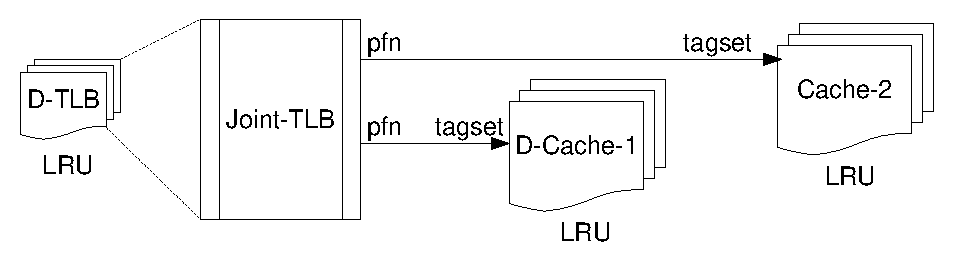
\includegraphics[width=0.8\textwidth]{4.analysis/mips}\\
  \caption{Схема MMU микропроцессора MIPS}\label{mips_mmu_scheme}
\end{figure}

По шагам подготовки генератора тестовых программ:
\begin{enumerate}
  \item\label{step_mmu} структура MMU построена, для этого пришлось ознакомиться с
  документацией по архитектуре микропроцессора~\cite{mips64_III},
  это заняло 1 человеко-день;
  \item\label{step_procedures}
  на основе анализа системы команд архитектуры MIPS~\cite{mips64_II}
  были выделены следующие процедуры для описания тестовых
  ситуаций:\\
  AddressTranslation, LoadMemory, StoreMemory, BytesSelect,
  BytesExpand -- на это ушел 1 человеко-день;
  \item в генераторе ограничений был использован зеркальный метод
  генерации ограничений для кэшируемых неотображаемых обращений и
  совместно-зеркальный метод генерации ограничений для остальных
  обращений -- на это ушло с учетом отладки 5 человеко-дней;
  \item для процедуры AddressTranslation в виде ограничений была
  записана модель виртуальной памяти (виды обращений в разных
  областях виртуальной памяти -- кэшируемое или некэшируемое,
  отображаемое или неотображаемое), для процедуры LoadMemory в виде
  ограничений были записаны взаимосвязи физических адресов и
  считанных из основной памяти данных (см.
  п.~\ref{module_algorithm} диссертации), для процедур BytesSelect и
  BytesExpand был выписан перебор значений младших бит физического
  адреса и границ части нужной длины двойного слова, являющего
  результатом чтения из памяти или записи в память -- с учетом
  отладки на это ушло 3 человеко-дня;
  \item\label{step_testsituations}
   по результатам знакомства с документацией по системе команд
  архитектуры MIPS~\cite{mips64_II} было выделено 8 инструкций
  (load / store --- byte / halfword / word / doubleword), в каждой инструкции по
  2 тестовые ситуации (AddressError(невыровненный виртуальный
  адрес) / полное выполнение инструкции), на подготовку описаний
  тестовых ситуаций ушло 1 человеко-день;
  \item\label{step_z3} использовался решатель ограничений Z3~\cite{Z3}, который
  печатал модель в виде пар <<(имя, значение)>>, среди имен
  выбирались начальные значения регистров и инициализирующие тегсеты
  кэшируемых неотображаемых обращений, по которым генерировались
  инициализирующие инструкции -- с учетом отладки на это ушло 1
  человеко-день;
  \item\label{step_compose} были объединены имеющиеся компоненты чтения описаний
  тестовых ситуаций и построения ограничений для операторов
  \texttt{let} и \texttt{assert} и новые компоненты, описывающие
  последовательности тестовых ситуаций в кэш-памяти и TLB,
  описывающие процедуры описаний тестовых ситуаций и генерирующие
  искомую тестовую программу -- на это ушло 1 человеко-день.
\end{enumerate}

Итого на построение генератора тестовых программ для MIPS ушло около
2,5 человеко-недель. При этом при построении генератора тестовых
программ для другого микропроцессора архитектуры MIPS (он может
отличаться количественными параметрами кэширующих буферов, размерами
виртуальных и физических адресов) повторно можно использовать
результаты шагов \ref{step_mmu}, \ref{step_procedures},
\ref{step_testsituations}, \ref{step_z3} и \ref{step_compose},
остальные шаги выполняются аналогичным образом с заменой
количественных параметров . Это позволяет достичь уровень
переиспользования в 40\% ($\frac{5 * 100\%}{13}$). Ручное создание
генератора тестовой программы для микропроцессора MIPS RM7000
~\cite{kamkin} заняло в сумме 2 человеко-месяца. Данные о
трудоемкости показывают, что при сходной полноте тестового набора
представленные в диссертации методы позволяют сократить время
построения генератора тестовых программ более чем в 3 раза.

Был подготовлен прототип генератора тестовых программ для
микропроцессора архитектуры MIPS. Были проведены эксперименты по
генерации тестовых программ на массивах тестовых шаблонов. Первый
набор экспериментов был связан с исследованием вероятности того, что
ограничения, построенные по методу совместной генерации, будут
совместны и дадут искомую тестовую программу. В таблице~\ref{exps1}
приведены результаты этих экспериментов для тестовых шаблонов из
двух инструкций. Таких тестовых шаблонов с различными
неэквивалентными зависимостями по данным было 240. Из них 15\%
несовместных тестовых шаблонов (для них не может существовать ни
одна тестовая программа). Остальные 85\% тестовых шаблонов составили
основу экспериментов. Были подготовлены начальные состояния
микропроцессора двух типов: произвольные (значения тегов в ячейках
кэш-памяти были сгенерированы случайным образом) и подготовленные
(значения тегов в ячейках были выбраны так, чтобы они с большей
вероятностью пересекались с номерами физических кадров состояния
TLB).

\begin{table}[h]
  \begin{tabular}{|c|c|c|c|c|}
  \hline
  \begin{tabular}{c}тип\\начального\\состояния\end{tabular}&
  \begin{tabular}{c}доля\\реали-\\зованных\\тестовых\\шаблонов\end{tabular}&
  \begin{tabular}{c}доля\\нереализо-\\ванных\\тестовых\\шаблонов\end{tabular}&
  \begin{tabular}{c}КПД\\совместной\\генерации\end{tabular}&
  \begin{tabular}{c}общее\\время\\генерации\end{tabular}\\
  \hline \hline
  подготовленное & 49~\% & 36~\% & 58~\% & 85~с. \\
  \hline
  произвольное & 32~\% & 53~\% & 38~\% & 170~с. \\
  \hline
  \end{tabular}
  \caption{Эксперименты с совместной генерацией; $n$ =
  2}\label{exps1}
\end{table}

Эксперименты показали, что использование совместной генерации на
произвольных начальных данных дает возможность построить тестовые
программы для 35-40\% тестовых шаблонов с различными зависимостями
по регистрам; на подготовленных начальных данных применением
совместной генерации удается достичь 55-60\% покрытия для тестовых
шаблонов. Важны оба случая, поскольку при первом запуске состояние
микропроцессора будет произвольным, а при всех последующих запусках
состояния, полученных от прошлых запусков, будут уже подготовленными
--- тем самым повысится вероятность построения тестовой программы по
ограничениям, сгенерированным методом совместной генерации.
Зеркальным методом (в силу его полноты) удалось построить тестовые
программы для всех тестовых совместных шаблонов. На все тестовые
шаблоны <<зеркальному методу>> потребовалось около 220 секунд.

%% посмотреть n = 3 и n = 4

%% посмотреть максимальную длину минимальной необходимой длины
%% инициализирующей последовательности для зеркальной генерации

\section{Генерация ограничений для архитектуры PowerPC}

\begin{utv}
Для архитектуры PowerPC возможно применение применение методов
генерации ограничений, описыванных в диссертации, для генерации
тестовых программ по тестовым шаблонам; причем методов достаточно
для полного описания поведения MMU микропроцессоров архитектуры
PowerPC.
\end{utv}

Рассмотрим исполнение инструкции обращения к памяти в
микропроцессоре архитектуры PowerPC~\cite{shnitman}. MMU в
микропроцессорах PowerPC включает в себя (количественные
характеристики приведены для микропроцессора PowerPC 970FX
~\cite{PowerPC970FXUserManual} -- см.
рис.~\ref{powerpc_mmu_scheme}):
\begin{itemize}
  \item \emph{кэш-память данных первого уровня (D-Cache-1)}: размер 32
килобайта, наборно-ассоциативная кэш-память, количество секций равно
2, размер строки кэш-памяти 128 байт, effective index real tag,
стратегия вытеснения \LRU;
  \item \emph{кэш-память второго уровня (Cache-2)}: размер 512
  килобайт, наборно-ассоциативная кэш-память, количество секций
  равно 8, стратегия вытеснения LRU, размер строки кэш-памяти 128
  байт, real index real tag;
  \item \emph{кэш-буфер TLB (D-TLB)}: наборно-ассоциативный буфер,
  количество секций 4, количество наборов в каждой секции 256;
  стратегия вытеснения LRU;
  \item \emph{таблица страниц виртуальной памяти (PageTable)}: размер
  виртуального адреса 65 бит, размер физического адреса 42 бита;
  \item \emph{сегментные регистры (SLB)}: полностью ассоциативный
  буфер, размер 64 строки;
  \item \emph{буфер непосредственной трансляции адресов (D-ERAT)}:
  наборно-ассоциативный буфер, количество секций равно 2, в каждой
  секции по 64 строки; стратегия вытеснения \FIFO.
\end{itemize}
Таким образом, проблема возникнет при записи ограничений на
кэш-память и на TLB.

Инструкция может содержать тестовые ситуации в:
\begin{itemize}
  \item кэш-памяти данных первого уровня, первого и второго уровней;
  \item кэш-буфере данных TLB (D-TLB);
  \item кэш-буфере непосредственной трансляции адресов (D-ERAT).
\end{itemize}

\begin{figure}[h] \center
  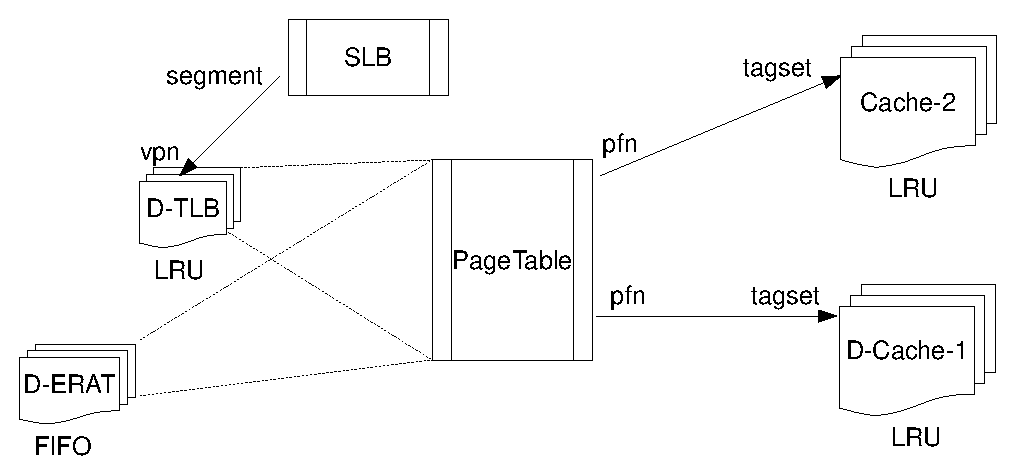
\includegraphics[width=0.8\textwidth]{4.analysis/ppc}\\
  \caption{Схема MMU микропроцессора PowerPC 970FX}\label{powerpc_mmu_scheme}
\end{figure}

Совместная генерация возможна (см. рис.~\ref{powerpc_mmu_scheme}):
\begin{itemize}
  \item на границе D-ERAT--кэш-память, так как получаемый из D-ERAT номер
физического кадра (pfn) становится битовым полем тегсета физического
адреса;
  \item на границе SLB--D-TLB, так как значение сегментного регистра
  становится битовым полем номера страницы виртуальной памяти (vpn);
  \item на границе D-TLB--кэш-память, так как получаемый из D-TLB номер
физического кадра (pfn) становится битовым полем тегсета физического
адреса.
\end{itemize}

\section{Генерация ограничений для архитектуры Alpha}

\begin{utv}
Для архитектуры Alpha возможно применение применение методов
генерации ограничений, описыванных в диссертации, для генерации
тестовых программ по тестовым шаблонам.
\end{utv}

Рассмотрим исполнение инструкции обращения к памяти в
микропроцессоре архитектуры Alpha. MMU в микропроцессорах Alpha
включает в себя  (количественные характеристики приведены для
микропроцессора Alpha 21264~\cite{HennessyPatterson3rd} -- см.
рис.~\ref{alpha_mmu_scheme}):
\begin{itemize}
  \item \emph{кэш-память данных первого уровня (D-Cache-1)}:
  virtually indexed physically tagged, размер 64 килобайта,
  наборно-ассоциативный, количество секций равно 2, стратегия вытеснения
  \LRU, размер строки кэш-памяти 64 байта;
  \item \emph{кэш-память второго уровня (Cache-2)}: physically
  indexed physically tagged, прямого отображения, размер от 1 до 16
  мегабайт
  \item \emph{таблица TLB (D-TLB)}: 128 строк, полностью
  ассоциативная, размер виртуального адреса 48/43 бит, размер физического адреса
  44/41 бит, размер страницы виртуальной памяти от 8 килобайт до 4
  мегабайт;
  \item \emph{буфер вытесненных данных (VictimBuffer)}: полностью
  ассоциативный, количество строк равно 8, стратегия
  вытеснения \FIFO.
\end{itemize}
Таким образом, основная проблема при записи ограничений -- большой
размер содержимого кэш-памяти.

Инструкция может содержать тестовые ситуации в:
\begin{itemize}
  \item кэш-памяти данных первого уровня;
  \item кэш-памяти первого и второго уровней.
\end{itemize}

\begin{figure}[h] \center
  \includegraphics[width=0.8\textwidth]{4.analysis/alpha}\\
  \caption{Схема MMU микропроцессора Alpha}\label{alpha_mmu_scheme}
\end{figure}

Совместная генерация возможна на границе TLB--кэш-память, так как
получаемый из TLB номер физического кадра (pfn) становится битовым
полем тегсета физического адреса (см.рис.~\ref{alpha_mmu_scheme}).



\section{Генерация ограничений для архитектуры Pentium}

\begin{utv}
Для архитектуры Pentium возможно применение применение методов
генерации ограничений, описыванных в диссертации, для генерации
тестовых программ по тестовым шаблонам.
\end{utv}

Рассмотрим исполнение инструкции обращения к памяти в
микропроцессоре архитектуры Pentium P6. MMU в микропроцессорах
Pentium включает в себя (количественные характеристики приведены для
микропроцессора Intel Pentium III~\cite{HennessyPatterson3rd} -- см.
рис.~\ref{p6_mmu_scheme}):
\begin{itemize}
  \item \emph{кэш-память данных первого уровня (D-Cache-1)}: размер
  16 килобайт, наборно-ассоциативная, количество секций равно 2,
  стратегия вытеснения \LRU, размер строки 32 байта;
  \item \emph{кэш-память второго уровня (Cache-2)}: размер от 256 килобайт
  до 2 мегабайт, наборно-ассоциативная, количество секций равно 8, стратегия
  вытеснения \LRU, размер строки 32 байта;
  \item \emph{кэш-буфер TLB (D-TLB)}: наборно-ассоциативный,
  количество секций равно 4, в каждой секции 16 строк, стратегия вытеснения
  \PseudoLRU;
  \item \emph{таблица страниц виртуальной памяти (PageTable)}:
  размер страницы от 8 килобайт, длина логического адреса 48 бит,
  длина линейного адреса 32 бита, длина физического адреса 32 бита;
  \item \emph{таблица дескрипторов сегментов (SDT)}: размер от 8 байт до 64
  килобайт~\cite{FundamentalOfComputerOrganizationAndDesign}.
\end{itemize}
Таким образом, проблема возникнет при записи ограничений на
кэш-память и на TLB.

Инструкция может содержать тестовые ситуации в:
\begin{itemize}
  \item кэш-памяти данных первого уровня, первого и второго уровней;
  \item кэш-буфере данных TLB (D-TLB).
\end{itemize}

\begin{figure}[h] \center
  \includegraphics[width=0.8\textwidth]{4.analysis/p6}\\
  \caption{Схема MMU микропроцессора Pentium}\label{p6_mmu_scheme}
\end{figure}

Совместная генерация возможна (см. рис.~\ref{p6_mmu_scheme}):
\begin{itemize}
  \item на границе SDT--D-TLB, так как значение сегментного регистра
  становится битовым полем номера страницы виртуальной памяти (vpn);
  \item на границе D-TLB--кэш-память, так как получаемый из D-TLB номер
физического кадра (pfn) становится битовым полем тегсета физического
адреса;
  \item на границе SDT--кэш-память при неотображаемом обращении, так как
  получаемый из SDT сегментный регистр становится битовым полем тегсета физического
адреса.
\end{itemize}


%! добавить еще результаты экспериментов! :)

% !Mode:: "TeX:UTF-8"
\chapter*{Заключение}
\addcontentsline{toc}{chapter}{Заключение}

Основные научные и практические результаты, полученные в
диссертационной работе и выносимые на защиту, состоят в следующем:

\Results

%Основные результаты диссертации являются новыми, получены автором самостоятельно.




\pagebreak
\appendix
% !Mode:: "TeX:UTF-8"
\chapter{Таблицы ограничений}
%\addcontentsline{toc}{chapter}{Приложение А: Таблицы ограничений}

\begin{table}[h] \small
\begin{tabular}{|c|c|c|c|}
\hline  & \centering случай &
\begin{tabular}{c}переменная\\перебора\end{tabular} & система \\
\hline \hline \multirow{10}{*}{\rotatebox{90}{кэш-попадание}} &
\makecell[c{p{0.3\textwidth}}]{тегсет находится в начальном
состоянии буфера, к нему нет обращений до данной инструкции и он всё
ещё не вытеснен} & $\lambda \in L_0$ &
$\left\{\begin{array}{l} x = \lambda\\
x \notin \{x_1, ..., x_n\}\\
\bigwedge\limits_{x_m:\mbox{miss}}\sum\limits_{i=1}^W v_m(\xi_i) +
\sum\limits^{m-1}_{i=1} u_m(x_i) < W
\end{array}\right.
$ \\ \hhline{~|---} & \makecell[c{p{0.3\textwidth}}]{тегсет
находится в начальном состоянии буфера, к нему есть обращение до
данной инструкции и он всё ещё не вытеснен} & $\lambda \in L_0$ &
$\left\{\begin{array}{l} x = \lambda\\
x \in \{x_1, ..., x_n\}\\
\bigwedge\limits_{x_m:\mbox{miss}}\sum\limits^{m-1}_{i=1} u_m(x_i) <
W
\end{array}\right.
$ \\  \hhline{~|---} & \makecell[c{p{0.3\textwidth}}]{тегсет был
внесен одним из кэш-промахов и с того момента не вытеснен} & -- &
$\left\{\begin{array}{l}
x \in [x_1, ..., x_n]_{miss}\\
\bigwedge\limits_{x_m:\mbox{miss}}\sum\limits^{m-1}_{i=1} u_m(x_i) <
W
\end{array}\right.
$ \\ \hline \hline \multirow{20}{*}{\rotatebox{90}{кэш-промах}} &
\makecell[c{p{0.3\textwidth}}]{тегсет встречается впервые} & -- &
$\left\{\begin{array}{l} x \notin L_0\\
x \notin [x_1, ..., x_n]_{miss}\\
\end{array}\right.
$ \\ \hhline{~|---} & \makecell[c{p{0.3\textwidth}}]{тегсет ранее
был внесен одной из инструкций шаблона, затем вытеснен} & -- &
$\left\{\begin{array}{l}
x \in [x_1, ..., x_n]_{miss}\\
\bigvee\limits_{x_m : \mbox{miss}}\sum\limits^{m-1}_{i=1} u_m(x_i) \geqslant W\\
\end{array}\right.$ \\  \hhline{~|---} &
\makecell[c{p{0.3\textwidth}}]{тегсет находился в начальном
состоянии буфера и был вытеснен, к нему не было обращений в шаблоне}
& $\lambda \in L_0$ & $\left\{\begin{array}{l}
x = \lambda\\
x \notin \{x_1, ..., x_n\}\\
\bigvee\limits_{x_m : \mbox{miss}}\sum\limits^W_{i=1} v_m(\xi_i) + \sum\limits^{m-1}_{i=1} u_m(x_i) \geqslant W\\
\end{array}\right.
$ \\ \hhline{~|---} & \makecell[c{p{0.3\textwidth}}]{тегсет
находился в начальном состоянии буфера и был вытеснен, к нему было
обращение в шаблоне после последнего внесения в буфер} & $\lambda
\in L_0$ &
$\left\{\begin{array}{l} x = \lambda\\
x \in \{x_1, ..., x_n\}\\
\bigvee\limits_{x_m : \mbox{miss}}\sum\limits^{m-1}_{i=1} u_m(x_i) \geqslant W\\
\end{array}\right.
$ \\ \hline
\end{tabular}
\caption{Таблица систем уравнений в случае стратегии вытеснения
\PseudoLRU c использованием функций полезности}\label{plru_table}
\end{table}


\begin{landscape}
\begin{table}[p]\small
\begin{tabular}{|c|c|c|c|c|c|}
\hline  & \centering случай &
\begin{tabular}{c}переменная\\перебора\end{tabular} & система &
\begin{tabular}{c}функция полезности\\для кэш-попадания\end{tabular} &
\begin{tabular}{c}функция полезности\\для кэш-промаха\end{tabular} \\
\hline \hline \multirow{10}{*}{\rotatebox{90}{кэш-попадание}} &
\makecell[c{p{0.38\textwidth}}]{тегсет находится в начальном
состоянии буфера, к нему нет обращений до данной инструкции и он всё
ещё не вытеснен} & $\lambda_\delta \in D$ &
$\left\{\begin{array}{l} x = \lambda_\delta\\
x \notin \{x_1, ..., x_n\}\\
\sum\limits^n_{i=1} u(x_i) \leqslant w - \delta
\end{array}\right.
$ &
\begin{tabular}{c}
$x_i \in \{ \lambda_{\delta+1}, ..., \lambda_w\}$\\
$\wedge~x_i \notin \{x_1, ..., x_{i-1}\}$
\end{tabular}
& $R(x_i) = R(x)$
\\ \hhline{~|-----}
& \makecell[c{p{0.38\textwidth}}]{тегсет находится в начальном
состоянии буфера, к нему есть обращение до данной инструкции и он
всё ещё не вытеснен} & $\lambda_\delta \in D$ &
$\left\{\begin{array}{l} x = \lambda_\delta\\
x \in \{x_1, ..., x_n\}\\
\sum\limits^n_{i=1} u(x_i) < w
\end{array}\right.
$ &
\begin{tabular}{c}
$x \notin \{x_i, ..., x_n\}~\wedge$\\
$x_i \in \{ \lambda_{\delta+1}, ..., \lambda_w\}$\\
$\wedge~x_i \notin \{ x_{i+1}, ..., x_n\}$\\
\end{tabular}
&
\begin{tabular}{c}
$x \notin \{x_i, ..., x_n\}$\\
$\wedge~R(x_i) = R(x)$\\
\end{tabular}
\\  \hhline{~|-----}
& \makecell[c{p{0.38\textwidth}}]{тегсет был внесен одним из
кэш-промахов и с того момента не вытеснен} & -- &
$\left\{\begin{array}{l} x \in [x_1, ..., x_n]_{miss}\\
\sum\limits^n_{i=1} u(x_i) < w
\end{array}\right.
$ &
\begin{tabular}{c}
$x \notin \{x_i, ..., x_n\}$\\
$\wedge~R(x_i) = R(x)~\wedge$\\
$x_i \notin \{ x_{i+1}, ..., x_n\}$\\
\end{tabular}
&
\begin{tabular}{c}
$x \notin \{x_i, ..., x_n\}$\\
$\wedge~R(x_i) = R(x)$\\
\end{tabular}
\\ \hline \hline \multirow{15}{*}{\rotatebox{90}{кэш-промах}}
& \makecell[l]{тегсет встречается впервые} & -- &
$\left\{\begin{array}{l} x \notin D\\
x \notin [x_1, ..., x_n]_{miss}\\
\end{array}\right.
$ & -- & -- \\ \hhline{~|-----} &
\makecell[l{p{0.38\textwidth}}]{тегсет ранее был внесен одной из
инструкций шаблона, затем вытеснен} & -- & $\left\{\begin{array}{l}
x \in [x_1, ..., x_n]_{miss}\\
\sum\limits^n_{i=1} u(x_i) \geqslant w\\
\end{array}\right.$ &
\begin{tabular}{c}
$x \notin \{x_i, ..., x_n\}$\\
$\wedge~R(x_i) = R(x)~\wedge$\\
$x_i \notin \{ x_{i+1}, ..., x_n\}$\\
\end{tabular}
&
\begin{tabular}{c}
$x \notin \{x_i, ..., x_n\}$\\
$\wedge~R(x_i) = R(x)$\\
\end{tabular}
\\  \hhline{~|-----} &
\makecell[c{p{0.38\textwidth}}]{тегсет находился в начальном
состоянии буфера и был вытеснен, к нему не было обращений в шаблоне}
& $\lambda_\delta \in D$ &
$\left\{\begin{array}{l} x = \lambda_\delta\\
x \notin \{x_1, ..., x_n\}\\
\sum^n_{i=1} u(x_i) \geqslant w - \delta + 1\\
\end{array}\right.
$ &
\begin{tabular}{c}
$x_i \in\{\lambda_{\delta+1}, ..., \lambda_w\}$\\
$\wedge~x_i \notin \{x_1, ..., x_{i-1}\}$\\
\end{tabular}
&
\begin{tabular}{c}
$R(x_i) = R(x)$\\
\end{tabular}
\\ \hhline{~|-----} &
\makecell[c{p{0.38\textwidth}}]{тегсет находился в начальном
состоянии буфера и был вытеснен, к нему было обращение в шаблоне
после последнего внесения в буфер} & $\lambda_\delta \in D$ &
$\left\{\begin{array}{l} x = \lambda_\delta\\
x \in \{x_1, ..., x_n\}\\
\sum\limits^n_{i=1} u(x_i) \geqslant w\\
\end{array}\right.
$ &
\begin{tabular}{c}
$x \notin \{x_i, ..., x_n\}~\wedge$\\
$x_i \in \{\lambda_{\delta+1}, ..., \lambda_w\}$\\
$\wedge x_i \notin \{ x_{i+1}, ..., x_n\}$\\
\end{tabular}
&
\begin{tabular}{c}
$x \notin \{x_i, ..., x_n\}$\\
$\wedge~R(x_i) = R(x)$\\
\end{tabular}
\\ \hline
\end{tabular}
\caption{Таблица систем уравнений для тестовых ситуаций в \LRU
кэширующих буферах c использованием функций
полезности}\label{hit_miss_table}
\end{table}
\end{landscape}

\begin{landscape}
\begin{table}
\begin{tabular}{|c|c|c|c|c|c|}
\hline  & \centering случай &
\begin{tabular}{c}переменная\\перебора\end{tabular} & система &
\begin{tabular}{c}функция\\полезности\\для кэш-\\попадания\end{tabular} &
\begin{tabular}{c}функция\\полезности\\для кэш-\\промаха\end{tabular} \\
\hline \hline \rotatebox{90}{кэш-попадание} & -- & -- & -- & -- & --
\\ \hline \hline \multirow{15}{*}{\rotatebox{90}{кэш-промах}} &
\makecell[c{p{0.35\textwidth}}]{тегсет встречается впервые} & -- &
$\left\{\begin{array}{l} x \notin D\\
x \notin [x_1, ..., x_n]_{miss}\\
\end{array}\right.
$ & -- & -- \\ \hhline{~|-----} &
\makecell[c{p{0.35\textwidth}}]{тегсет ранее был внесен одной из
инструкций шаблона, затем вытеснен} & -- & $\left\{\begin{array}{l}
x \in [x_1, ..., x_n]_{miss}\\
\left[ \sum\limits^n_{i=1} \right]_{miss} u(x_i) \geqslant w - \delta + 1\\
\end{array}\right.$& -- &
\begin{tabular}{c}
$x \notin \{x_i, ..., x_n\}$\\
$\wedge~R(x_i) = R(x)$\\
\end{tabular}
\\  \hhline{~|-----} &
\makecell[c{p{0.35\textwidth}}]{тегсет находился в начальном
состоянии буфера и был вытеснен, к нему не было обращений в шаблоне}
& $\lambda_\delta \in D$ &
$\left\{\begin{array}{l} x = \lambda_\delta\\
x \notin \{x_1, ..., x_n\}\\
\left[ \sum\limits^n_{i=1} \right]_{miss} u(x_i) \geqslant w - \delta + 1\\
\end{array}\right.$ & -- &
\begin{tabular}{c}
$R(x_i) = R(x)$\\
\end{tabular}
\\ \hhline{~|-----} &
\makecell[c{p{0.35\textwidth}}]{тегсет находился в начальном
состоянии буфера и был вытеснен, к нему было обращение в шаблоне
после последнего внесения в буфер} & $\lambda_\delta \in D$ &
$\left\{\begin{array}{l} x = \lambda_\delta\\
x \in \{x_1, ..., x_n\}\\
\left[ \sum\limits^n_{i=1} \right]_{miss} u(x_i) \geqslant w\\
\end{array}\right.$ & -- &
\begin{tabular}{c}
$x \notin \{x_i, ..., x_n\}$\\
$\wedge~R(x_i) = R(x)$\\
\end{tabular}
\\ \hline
\end{tabular}
\caption{Таблица систем ограничений в случае стратегии вытеснения
\FIFO c использованием функций полезности}\label{fifo_table}
\end{table}
\end{landscape}

\begin{landscape}
\begin{table} \small
\begin{tabular}{|c|c|c|c|c|c|}
\hline  & \centering случай &
\begin{tabular}{c}переменная\\перебора\end{tabular} & система &
\begin{tabular}{c}функция полезности\\для кэш-попадания\end{tabular} &
\begin{tabular}{c}функция полезности\\для кэш-промаха\end{tabular} \\
\hline \hline \multirow{10}{*}{\rotatebox{90}{кэш-попадание}} &
\makecell[c{p{0.38\textwidth}}]{тегсет находится в начальном
состоянии буфера, к нему нет обращений до данной инструкции и он всё
ещё не вытеснен} & $\lambda_\delta \in D$ &
$\left\{\begin{array}{l} x = \lambda_\delta\\
x \notin \{x_1, ..., x_n\}\\
\sum\limits^n_{i=1} u(x_i) \leqslant w - \delta
\end{array}\right.
$ &
\begin{tabular}{c}
$x_i \in \{ \lambda_{\delta+1}, ..., \lambda_\Delta\}$\\
$\wedge~x_i \notin \{x_1, ..., x_{i-1}\}$
\end{tabular}
& $R(x_i) = R(x)$
\\ \hhline{~|-----}
& \makecell[c{p{0.38\textwidth}}]{тегсет находится в начальном
состоянии буфера, к нему есть обращение до данной инструкции и он
всё ещё не вытеснен} & $\lambda_\delta \in D$ &
$\left\{\begin{array}{l} x = \lambda_\delta\\
x \in \{x_1, ..., x_n\}\\
\sum\limits^n_{i=1} u(x_i) < w
\end{array}\right.
$ &
\begin{tabular}{c}
$x \notin \{x_i, ..., x_n\}~\wedge$\\
$x_i \in \{ \lambda_{\delta+1}, ..., \lambda_\Delta\}$\\
$\wedge~x_i \notin \{ x_{i+1}, ..., x_n\}$\\
\end{tabular}
&
\begin{tabular}{c}
$x \notin \{x_i, ..., x_n\}$\\
$\wedge~R(x_i) = R(x)$\\
\end{tabular}
\\  \hhline{~|-----}
& \makecell[c{p{0.38\textwidth}}]{тегсет был внесен одним из
кэш-промахов и с того момента не вытеснен} & -- &
$\left\{\begin{array}{l} x \in [x_1, ..., x_n]_{miss}\\
\sum\limits^n_{i=1} u(x_i) < w
\end{array}\right.
$ &
\begin{tabular}{c}
$x \notin \{x_i, ..., x_n\}$\\
$\wedge~R(x_i) = R(x)~\wedge$\\
$x_i \notin \{ x_{i+1}, ..., x_n\}$\\
\end{tabular}
&
\begin{tabular}{c}
$x \notin \{x_i, ..., x_n\}$\\
$\wedge~R(x_i) = R(x)$\\
\end{tabular}
\\ \hline \hline \multirow{20}{*}{\rotatebox{90}{кэш-промах}}
& \makecell[c{p{0.38\textwidth}}]{тегсет встречается впервые} & -- &
$\left\{\begin{array}{l} x \notin D\\
x \notin [x_1, ..., x_n]_{miss}\\
\end{array}\right.
$ & -- & -- \\ \hhline{~|-----} &
\makecell[c{p{0.38\textwidth}}]{тегсет ранее был внесен одной из
инструкций шаблона, затем вытеснен} & -- &
$\left\{\begin{array}{l} x \in [x_1, ..., x_n]_{miss}\\
\sum\limits^n_{i=1} u(x_i) \geqslant w\\
\end{array}\right.
$ &
\begin{tabular}{c}
$x \notin \{x_i, ..., x_n\}$\\
$\wedge~R(x_i) = R(x)~\wedge$\\
$x_i \notin \{ x_{i+1}, ..., x_n\}$\\
\end{tabular}
&
\begin{tabular}{c}
$x \notin \{x_i, ..., x_n\}$\\
$\wedge~R(x_i) = R(x)$\\
\end{tabular}
\\  \hhline{~|-----} &
\makecell[c{p{0.38\textwidth}}]{тегсет находился в начальном
состоянии буфера и был вытеснен, к нему не было обращений в шаблоне}
& $\lambda_\delta \in D$ &
$\left\{\begin{array}{l} x = \lambda_\delta\\
x \notin \{x_1, ..., x_n\}\\
\sum\limits^n_{i=1} u(x_i) \geqslant w - \delta + 1\\
\end{array}\right.
$ &
\begin{tabular}{c}
$x_i \in\{\lambda_{\delta+1}, ..., \lambda_\Delta\}$\\
$\wedge~x_i \notin \{x_1, ..., x_{i-1}\}$\\
\end{tabular}
&
\begin{tabular}{c}
$R(x_i) = R(x)$\\
\end{tabular}
\\ \hhline{~|-----} &
\makecell[c{p{0.38\textwidth}}]{тегсет находился в начальном
состоянии буфера и был вытеснен, к нему было обращение в шаблоне
после последнего внесения в буфер} & $\lambda_\delta \in D$ &
$\left\{\begin{array}{l} x = \lambda_\delta\\
x \in \{x_1, ..., x_n\}\\
\sum\limits^n_{i=1} u(x_i) \geqslant w\\
\end{array}\right.
$ &
\begin{tabular}{c}
$x \notin \{x_i, ..., x_n\}~\wedge$\\
$x_i \in \{\lambda_{\delta+1}, ..., \lambda_\Delta\}$\\
$\wedge~x_i \notin \{ x_{i+1}, ..., x_n\}$\\
\end{tabular}
&
\begin{tabular}{c}
$x \notin \{x_i, ..., x_n\}$\\
$\wedge~R(x_i) = R(x)$\\
\end{tabular}
\\ \hline
\end{tabular}
\caption{Таблица систем уравнений для тестовых ситуаций в \LRU
кэширующем буфере c <<грязными>> ячейками в начальном состоянии,
использующих функции полезности}\label{dirty_hit_miss_table}
\end{table}
\end{landscape}

% !Mode:: "TeX:UTF-8"
\chapter{Доказательства теорем и лемм}\label{sec:proofs}
%\addcontentsline{toc}{chapter}{Приложение А: Таблицы ограничений}

\begin{lemma}\label{QuantorElimination}
Для любых неотрицательных чисел $x$, $y$ и $N$ таких, что $0 \leqslant x, y < 2^N$, справедливо следующее (сравнения беззнаковые):
$$( \exists k \in \mathds{N} : x < 2^k \leqslant y ) \Leftrightarrow (y > x ~\wedge~ x \oplus y > x)$$
\end{lemma}
\begin{proof}
  // TODO
\end{proof}

\theoremtext{\ref{mirror_fullness_none}}{\FullnessMirrorNone}
\begin{proof}
  Особо подчеркну сначала, что в формулировке теоремы $n$ --- количество обращений к таблице в тестовом шаблоне. А в алгоритме построения ограничений $n$ --- количество \textbf{успешных} обращений к таблице в тестовом шаблоне. Чтобы согласовать обозначения, будем далее придерживаться обозначений из алгоритма: ключи в регионах с успешными обращениями обозначать как $k_i$, $R_i$ для $i = 1, 2, ..., n$, а ключа в регионах с неуспешными обращениями обозначать как $k'_j$, $R'_j$ для $j = 1, 2, ..., n'$ ($n$ в формулировке теоремы есть новое $n$ + $n'$).

  Обозначим $L$ --- состояние таблицы перед тестовым шаблоном. Тогда согласно посылке в условии теоремы для каждого допустимого $i$ выполнено: $(k_i || R_i) \in L$ --- и для каждого допустимого $j$ выполнено: $(k'_j || R'_j) \notin L$. Для всех инструкций состояние таблицы одно и то же, поскольку стратегия вытеснения есть \texttt{none} (промах лишь фиксируется, но не <<исправляется>>). Тем самым. $L \supseteq \{ (k_1||R_1), ..., (k_n||R_n) \}$. Отсюда следует, что для каждого допустимого $j$ $(k'_j||R'_j) \notin \{ (k_1||R_1), ..., (k_n||R_n) \}$.

  Кроме того, поскольку $L$ --- состояние таблицы перед тестовым шаблоном, то количество ключей в каждом регионе, которое может находиться в $L$ равно $w$ (по определению $w$). Но поскольку $L \supseteq \{ (k_1||R_1), ..., (k_n||R_n) \}$, то количество различных ключей в каждом регионе в последовательности $(k_i, R_i)$ не может быть больше $w$. Осталось показать, что это количество выражается формулой, представленной в алгоритме. Действительно, для получения количества различных ключей в том же регионе достаточно просматривать все ключи с начала и отсчитывать те из них, что встречаются впервые, т.е. не встречаются среди предыдущих ключей, что и выражено в формуле.

  Итак, если для щаблона в заданном начальном состоянии есть какая-нибудь последовательность ключей в регионах, то система ограничений будет совместна, поскольку на этих же ключах и регионах выполнены ограничения, генерируемые согласно алгоритму.
\end{proof}

\theoremtext{\ref{mirror_fullness}}{\FullnessMirror}
\begin{proof}
Докажем даже более сильное утверждение (из него очевидно будет следовать требуемое в теореме): есть начальное состояние таблицы $L_0$, для него существуют такие $k_1, k_2, ..., k_n$, $R_1, R_2, ..., R_n$, что выполнены все $S_i$ и $P$; спрашивается, будут ли существовать такие $t_1, t_2, ..., t_m$, $r_1, r_2, ..., r_m$, что составленные ограничения (для тех же $k_1, k_2, ..., k_n$, $R_1$, $R_2$, ..., $R_n$) будут выполнены. Весь вопрос в том, как выбрать $t_1, t_2, ..., t_m$, $r_1, r_2, ..., r_m$. Доказательство можно разделить на две части: в первой будет предложен способ выбора $t_1, t_2, ..., t_m$, $r_1, r_2, ..., r_m$, а во второй будет показано, что на них выполняются ограничения.

\paragraph{выбор инициализирующей последовательности} предлагается делать\\следующим образом. Она будет состоять из подпоследовательностей $s_R$ для каждого $R$ из \textbf{множества} $\{R_1, R_2, ..., R_n\}$. Далее рассматривается построение такой подпоследовательности для произвольного $R$. Выберем из $L_0$ ключи, хранящиеся в регионе $R$, ровно в том порядке, в каком они там находятся (речь идет о порядке в смысле перестановок в таблицах вытеснения). Обозначим эту последовательность $V \equiv \langle v_1, v_2, ..., v_q \rangle$. Далее, удалим из последовательности $k_1, k_2, ..., k_n$ те ключи, чьи регионы не равны $R$, и те, которые присутствуют в последовательности $v_1, v_2, ..., v_q$. Обозначим получившуюся последовательность $U \equiv \langle u_1, u_2, ..., u_p\rangle$. Если $p < w$, то выберем $p{-}w$ произвольных ключей, не встречающихся в последовательностях $U$ и $V$. Обозначим эту последовательность $Z$. Тогда $s_R$ будет являться конкатенацией последовательностей $Z$, $U$ и $V$ (именно в этом порядке). Порядок конкатенации последовательностей $s_R$ произвольный. Последовательность $r_1, r_2, ..., r_m$ выбирается в соответствии с выбором последовательности конкатенации $s_R$.

\paragraph{выполнение системы ограничений} По построению все $(t_1||r_1)$, $(t_2||r_2)$, ..., $(t_m||r_m)$ разные. Кроме того, поскольку на $(k_i, R_i)$ выполнены все условия в тестовом шаблоне, то для них выполнено условие количества различных пар (ключ, регион) в каждом регионе для каждой инструкции. Далее, поскольку последовательность $(t_i, r_i)$ оканчивается последовательностью, дублирующей $L_0$ и стратегия вытеснения является существенно вытесняющей, то после таких инициализирующих обращений состояние таблиц станет точно таким же, каким оно было до инициализирующих обращений. Это значит, что для $(k_i, R_i)$ выполнены ограничения <<быть вытесненным>> (они и есть $S_i$). И поскольку последовательность $(t_1, r_1)$, $(t_2, r_2)$, .., $(t_m, r_m)$ содержит все $(k_1, R_1)$, ..., $(k_n, R_n)$, то выполнены ограничения\\$(k_i||R_i) \in \{(t_1||r_1), (t_2||r_2), ..., (t_m||r_m), (k_1||R_1), (k_2||R_2), ..., (k_{i-1}||R_{i-1})\}$.
\end{proof}

\begin{lemma}\label{PseudoLRUNolDisplacing}
Рассматривается последовательность промахов при стратегии вытеснения \PseudoLRU. Тогда в результате $w{-}1$ промаха строка региона на позиции 0 не будет вытеснена.
\end{lemma}
\begin{proof}
    Доказательство для лучшей читабельности приведено для случая $w = 8$, хотя всё аналогичное переносится на случай произвольного $w = 2^W$.

    Последняя строка таблицы вытеснения для \PseudoLRU имеет вид:\\$(m~6~4~5~0~1~2~3)$. Если разложить каждую позицию в битовую строку, то эту же перестановку можно задать следующим образом:
    \begin{itemize}
        \item элемент с позиции $x \in \{\bigl(\begin{smallmatrix}0\\0\\0
\end{smallmatrix}\bigr), \bigl(\begin{smallmatrix}0\\0\\1
\end{smallmatrix}\bigr), \bigl(\begin{smallmatrix}0\\1\\0
\end{smallmatrix}\bigr), \bigl(\begin{smallmatrix}0\\1\\1
\end{smallmatrix}\bigr)\}$ перемещается на позицию $x \oplus \bigl(\begin{smallmatrix}1\\0\\0
\end{smallmatrix}\bigr)$;
        \item элемент с позиции $x \in \{\bigl(\begin{smallmatrix}1\\0\\0
\end{smallmatrix}\bigr), \bigl(\begin{smallmatrix}1\\0\\1
\end{smallmatrix}\bigr)\}$ перемещается на позицию $x \oplus \bigl(\begin{smallmatrix}1\\1\\0
\end{smallmatrix}\bigr)$;
        \item элемент с позиции $x \in \{\bigl(\begin{smallmatrix}1\\1\\0
\end{smallmatrix}\bigr)\}$ перемещается на позицию $x \oplus \bigl(\begin{smallmatrix}1\\1\\1
\end{smallmatrix}\bigr)$;
        \item $m$ помещается на позицию 0.
\end{itemize}

Сокращая обозначения, перефразируем это:
\begin{itemize}
    \item элемент с позиции $x = \bigl(\begin{smallmatrix}0\\X\\X\end{smallmatrix}\bigr)$ перемещается на позицию $x \oplus \bigl(\begin{smallmatrix}1\\0\\0 \end{smallmatrix}\bigr)$;
    \item элемент с позиции $x = \bigl(\begin{smallmatrix}1\\0\\X\end{smallmatrix}\bigr)$ перемещается на позицию $x \oplus \bigl(\begin{smallmatrix}1\\1\\0\end{smallmatrix}\bigr)$;
    \item элемент с позиции $x = \bigl(\begin{smallmatrix}1\\1\\0\end{smallmatrix}\bigr)$ перемещается на позицию $x \oplus \bigl(\begin{smallmatrix}1\\1\\1\end{smallmatrix}\bigr)$;
    \item $m$ помещается на позицию 0.
\end{itemize}

Перевернем каждый столбец. Получится следующий набор правил перемещения в результате промаха:
\begin{itemize}
    \item элемент с позиции $x = \bigl(\begin{smallmatrix}X\\X\\0\end{smallmatrix}\bigr)$ перемещается на позицию $x \oplus \bigl(\begin{smallmatrix}0\\0\\1 \end{smallmatrix}\bigr)$;
    \item элемент с позиции $x = \bigl(\begin{smallmatrix}X\\0\\1\end{smallmatrix}\bigr)$ перемещается на позицию $x \oplus \bigl(\begin{smallmatrix}0\\1\\1\end{smallmatrix}\bigr)$;
    \item элемент с позиции $x = \bigl(\begin{smallmatrix}0\\1\\1\end{smallmatrix}\bigr)$ перемещается на позицию $x \oplus \bigl(\begin{smallmatrix}1\\1\\1\end{smallmatrix}\bigr)$;
    \item $m$ помещается на позицию 0.
\end{itemize}

Под действием этих правил происходят $w{-}1$ перемещений с <<перевернутой>> позиции $\bigl(\begin{smallmatrix}0\\0\\0\end{smallmatrix}\bigr)$. Покажем, что это перемещение имеет очень простой вид: 0, 1, 2, ... . Докажем по индукции. База очевидна: позиция изначально равна 0. Индуктивный переход. За позицией $2k$ будет следовать позиция $2k+1$ под действием первого правила. За позицией $2k+1$ будет следовать позиция $2k+2$ под действием остальных правил (0 и последовательность единичных битов инвертируется, что и есть прибавление единицы).

А если перемещение имеет такой вид, то за $w{-}1$ перемещение ни одна из <<перевернутых>> позиций (а, значит, и просто позиций) не равна $w{-}1$ (0, 1, 2, ..., $w{-}2$). А позиция $w{-}1$ --- это и есть позиция вытеснения согласно последней строке таблицы вытеснения для \PseudoLRU.
\end{proof}

\theoremtext{\ref{thm:PseudoLRU_essential}}{\PseudoLRUEssential}
\begin{proof}
    Из леммы~\ref{PseudoLRUNolDisplacing} следует, что первый внесенный в результате промаха $m$ не будет вытеснен после $w{-}1$ промахов. Однако при каждом промахе какие-то элементы вытесняются. Вносимые на каждом промахе $m$ проходят ту же <<траекторию>>, что и первый. Поэтому к ним снова применима лемма~\ref{PseudoLRUNolDisplacing}. Тем самым после $w$ промахов в регионе будет $w$ штук $m$. Но больше, чем $w$, и не может быть, поскольку это количество строк в регионе. Значит, после $w$ промахов весь регион будет состоять лишь из одних $m$.
\end{proof}

\theoremtext{\ref{thm_mirror_lenth_lru}}{\UpperBoundLRUMirror}
\begin{proof}
  Так же, как это было сделано при доказательстве
  теоремы~\ref{mirror_fullness}, разделим все $k_1, k_2, ..., k_n$
  по регионам. Для каждого задействованного региона составим свою
  инициализирующую последовательность (обозначим ее длину $m_i$
  для $i$'го задействованного региона) и сконкатенируем эти
  последовательности для получения искомой инициализирующей последовательности
   для всего тестового шаблона.
  Подпоследовательность последовательности $k_1, k_2, ..., k_n$,
  соответствующая одному региону, обозначим $y_1, y_2, ...,
  y_{n_i}$.

  Докажем, что $$m_i = M_i + w$$ где $M_i$ -- количество
  элементов последовательности $y_1, y_2, ..., y_{n_i}$, которые дают
  промахи при первых обращениях к ним. Тогда для всего тестового
  шаблона $m = \sum\limits_i m_i = \sum\limits_i M_i + \sum\limits_i w =
  M + w \cdot r$, где $r$ -- количество регионов, задействованных в
  $k_1, k_2, ..., k_n$. Очевидно, что $r \leqslant n$, тем самым это
  приводит к искомой оценке $m \leqslant M + n \cdot w$. Осталось
  доказать формулу для $m_i$.

  Укажем способ построения ключей инициализирующей последовательности. Выберем из $y_1, y_2, ..., y_{n_i}$ подпоследовательность,
  состоящую из тех ключей, которые дают промах и встречаются
  впервые. Обозначим их как $\mu \equiv \mu_1, \mu_2, ..., \mu_{MM_i}$. Они будут первыми ключами в   инициализирующей последовательности. Далее выберем из $y_1, y_2, ..., y_{n_i}$
  все ключи, при обращении к которым происходят попадания.
  Обозначим их как $\eta \equiv \eta_1, \eta_2, ..., \eta_{HH_i}$. Если $MM_i > 0$ и $MM_i +
  HH_i < w + 1$, выберем произвольные различные числа-ключи $\nu \equiv \nu_1, \nu_2,
  ..., \nu_{NN_i}$, которые не встречаются в $y_1, y_2, ..., y_{n_i}$. Итак, инициализирующая последовательность (для данного региона!) представляет собой конкатенацию последовательностей $\mu$, $\eta$ и $\nu$ (в этом порядке).

  Покажем, что такая инициализирующая последовательность удовлетворяет системе ограничений. Все ключи из тестового шаблона, при обращении к которым происходят попадания, встречаются в
  этой последовательности. Это следует из того, что первые такие ключи мы поместили явно (в конец последовательности), а дальнейшие ключи не могут встречаться впервые в тестовом шаблоне, в противном случае они были бы вытеснены до того, как должно быть попадание. Очевидно, что эти первые ключи не вытеснены, поскольку они помещены в конец инициализирующей последовательности. Все ключи, при обращении к которыми происходят промахи, тоже встречаются в этой последовательности (мы их туда поместили явно). При этом поскольку от своего промаха они отделены не менее $w+1$ инструкцией с разными ключами, то к моменту промаха они будут
  вытеснены (для первой инструкции это очевидно по построению, а
  для остальных следует из леммы~\ref{includedranges} о невложенных диапазонах вытеснения).

  Длина инициализирующей последовательности для шаблона без промахов (при $MM_i$ = 0) равна количеству ключей в $y_1, y_2, ..., y_{n_i}$, при обращении к
  которым происходят попадания. Их не более чем $w$,
  т.к. последовательность из попаданий может задать лишь часть
  или целиком весь регион. При $MM_i > 0$ длина последовательности
  есть сумма из $M_i$ (поскольку туда включаются все ключи $y_1, y_2,
  ..., y_{n_i}$, при обращении к которым происходят промахи) и
  $w$ (поскольку в инициализирующую последовательность добавляются фиктивные ключи и ключи, при обращении к которым происходят попадания). В обоих случах $m_i = M_i + w$.
\end{proof}

\theoremtext{\ref{thm_pseudoLRU_invariant}}{\PseudoLRUInvariant}
\begin{proof}
  Пусть происходит обращение с позицией $j = (j_1~j_2~\dots~j_W)$.
  Тогда согласно каноническому определению \PseudoLRU будет
  произведены следующие изменения: $B_{(1)} := j_1; B_{(1~j_1)} :=
  j_2; \dots B_{(1~j_1~j_2~\dots~j_{W-1})} := j_W$. Однако только
  часть этих изменений повлияет на
  $(\alpha_1~\alpha_2~\dots~\alpha_W)$, $\alpha_1 = B_{(1)}^{\neg
  i_1}, \alpha_2 = B_{(1~i_1)}^{\neg i_2}, \dots, \alpha_W =
  B_{(1~i_1~i_2~\dots~i_{W-1})}^{\neg i_W}$. А именно влияние будет
  на те элементы вектора, у которых совпадают индексы с изменяемыми
  элементами согласно каноническому определению. Иными словами,
  изменение $B_{(1~j_1~j_2~\dots~j_k)}$ будет влиять на
  $B_{(1~i_1~i_2~\dots~i_m)}$ тогда и только тогда, когда
  $(1~j_1~j_2~\dots~j_k) = (1~i_1~i_2~\dots~i_m)$. Докажем, что при
  этом $k = m$. Действительно, если $k > m$, то
  $(1~j_1~j_2~\dots~j_k) \geqslant 2^k$, а $(1~i_1~i_2~\dots~i_m) <
  2^{m+1} \leqslant 2^k$, что исключает равенство этих чисел.
  Аналогично доказывается невозможность случая $k < m$.

  Условие $(1~j_1~j_2~\dots~j_k) = (1~i_1~i_2~\dots~i_k)$
  эквивалентно условию $(j_1~j_2~\dots~j_k)$ $\oplus~(i_1~i_2~\dots~i_k) =
  0$. Переходя к полным векторам, это условие записывается в виде $(j_1~j_2~\dots~j_W) \oplus
  (i_1~i_2~\dots~i_W) < 2^{W-k+1}$. Или, переходя от векторов к
  числам, $i \oplus j < 2^{W-k+1}$.

  При этом изменение элементов вектора
  ($\alpha_1~\alpha_2~\dots~\alpha_W$) будет происходить следующим
  образом (используется определение степени через сложение по модулю
  2: $x^y \equiv x \oplus y \oplus 1$): $\alpha_k :=
  (B_{(1~j_1~j_2~\dots~j_{k-1})})^{\neg i_k} =
  (B_{(1~j_1~j_2~\dots~j_{k-1})}) \oplus (\neg i_k) \oplus 1 =
  B_{(1~j_1~j_2~\dots~j_{k-1})} \oplus i_k = j_k \oplus i_k$. Так
  как $(j_1~j_2~\dots~j_{k-1}) = (i_1~i_2~\dots~i_{k-1})$, то
  $(j_1~j_2~\dots~j_{k-2}) = (i_1~i_2~\dots~i_{k-2})$ и $i_{k-1} =
  j_{k-1}$. В таком случае изменяется и $\alpha_{k-1}$, причем
  $\alpha_{k-1} := i_{k-1} \oplus j_{k-1} = 0$. Аналогично
  рассуждая, получим, что $\alpha_{k-2} := 0,~\dots~\alpha_1 := 0$.
  Иными словами, возможно даже вычислить изменения предыдущих
  элементов -- всем им присваивается значение 0. Найдется такой $p$,
  что $i_1 = j_1~\wedge~i_2 = j_2~\wedge~i_{p-1} =
  j_{p-1}~\wedge~i_p \neq j_p$. В этом случае изменяется
  $\alpha_p$ следующим образом: $\alpha_p := i_p \oplus j_p = 1$.
  Или записывая это условие с использованием чисел $i$ и $j$: $2^{W-p} \leqslant i
  \oplus j < 2^{W-p+1}$.

  Таким образом, получаем, что для $i \oplus j \in
  [\frac{w}{2^k},~\frac{w}{2^{k-1}})$ будет произведены следующие
  присваивания: $\alpha_k := 1,~\alpha_{k-1} := 0,~\alpha_{k-2} :=
  0,~\dots~\alpha_1 := 0$, остальные элементы не будут изменены. Для
  $i \oplus j = 0$, т.е. $i = j$ все элементы $\alpha_k := i_k \oplus
  j_k = 0$. Причем изменение определяется только суммой по модулю 2
  чисел $i$ и $j$, что и является относительной позицией $j$
  относительно $i$.

  Осталось разобраться с ветвью вытесняемого ключа. Это будет такая
  позиция $i = (i_1~i_2~\dots~i_W)$, для которой справедливы
  уравнения $i_1 = \neg B_{k_1}~\wedge~i_2 = \neg
  B_{k_2}~\wedge~\dots~\wedge~i_W = \neg B_{k_W}$, где $k_1 = (1)$,
  $k_2 = (1~\neg B_{k_1})$, ..., $k_W = (1~\neg B_{k_1}~\neg
  B_{k_2}~\dots\\\neg B_{k_{W-1}})$. Используя уравнения для
  элементов $i$, можно переписать уравнения для элементов $k$
  следующим образом: $k_1 = (1)$,
  $k_2 = (1~i_1)$, ..., $k_W = (1~i_1~i_2~\dots~i_{W-1})$. Таким
  образом, элементы ветви вытесняемого ключа будут вычисляться
  следующим образом: $\alpha_m \equiv B_{(1~i_1~i_2~\dots~i_{m-1})}
  \oplus i_m \equiv B_{k_m} \oplus i_m \equiv \neg i_m \oplus i_m
  \equiv 1$. Иными словами, ветвь вытесняемого ключа состоит только
  из единиц.
\end{proof}


\pagebreak
%%%%\bibliographystyle{plain}
%%%%\bibliographystyle{gost71u}
\addcontentsline{toc}{chapter}{Литература}
\bibliographystyle{gost780s}
\bibliography{thesis}

%% привести оформление в соответствие с требованием: что-то всё время пропадает!

%%! добавить \cite{Pex}, \cite{symbolic_execution}

%%! вписать название препринта и номер тома

\end{document}
